% **************************************************
% Document Class Definition
% **************************************************
\documentclass[%
    paper=A4,					% paper size --> A4 is default in Germany
    twoside=true,				% onesite or twoside printing
    openright,					% doublepage cleaning ends up right side
    parskip=full,				% spacing value / method for paragraphs
    chapterprefix=true,			% prefix for chapter marks
    11pt,						% font size
    headings=normal,			% size of headings
    bibliography=totoc,			% include bib in toc
    listof=totoc,				% include listof entries in toc
    titlepage=on,				% own page for each title page
    captions=tableabove,		% display table captions above the float env
    draft=false,				% value for draft version
]{scrreprt}%

% **************************************************
% Debug LaTeX Information
% **************************************************
%\listfiles

% **************************************************
% Information and Commands for Reuse
% **************************************************
\newcommand{\thesisTitle}{Implementation and Semantics of an asynchronous evaluation engine for stream based specifications}
\newcommand{\thesisName}{Alexander Schramm}
\newcommand{\thesisSubject}{Master Thesis}
\newcommand{\thesisDate}{November 20, 2016}
\newcommand{\thesisVersion}{My First Draft}

\newcommand{\thesisFirstReviewer}{Prof. Dr. Martin Leucker}
\newcommand{\thesisFirstReviewerUniversity}{\protect{University of Luebeck}}
\newcommand{\thesisFirstReviewerDepartment}{Institute For Software Engineering and Programming Languages}

\newcommand{\thesisSecondReviewer}{Who Knöws}
\newcommand{\thesisSecondReviewerUniversity}{\protect{University of Luebeck}}
\newcommand{\thesisSecondReviewerDepartment}{We will see}

\newcommand{\thesisFirstSupervisor}{Cesar Sanchez}
% \newcommand{\thesisSecondSupervisor}{John Smith}

\newcommand{\thesisUniversity}{\protect{University of Luebeck}}
% \newcommand{\thesisUniversityDepartment}{Institute For Software Engineering and Programming Languages}
\newcommand{\thesisUniversityInstitute}{Institute For Software Engineering and Programming Languages}
% \newcommand{\thesisUniversityGroup}{Clean Thesis Group (CTG)}
\newcommand{\thesisUniversityCity}{Luebeck}
\newcommand{\thesisUniversityStreetAddress}{Ratzeburger Allee 160}
\newcommand{\thesisUniversityPostalCode}{23562}

% **************************************************
% Load and Configure Packages
% **************************************************
\usepackage[utf8]{inputenc}		% defines file's character encoding
\usepackage[english]{babel} % babel system, adjust the language of the content
\usepackage[					% clean thesis style
    figuresep=colon,%
    sansserif=false,%
    hangfigurecaption=false,%
    hangsection=true,%
    hangsubsection=true,%
    colorize=full,%
    colortheme=bluegreen,%
    bibsys=bibtex,%
    bibfile=Mendeley,%
    bibstyle=alphabetic,%
]{cleanthesis}
\usepackage{amssymb}
\usepackage{amsmath}
\bibliography{Mendeley}

\hypersetup{% setup the hyperref-package options
    pdftitle={\thesisTitle},	% 	- title (PDF meta)
    pdfsubject={\thesisSubject},% 	- subject (PDF meta)
    pdfauthor={\thesisName},	% 	- author (PDF meta)
    plainpages=false,			% 	-
    colorlinks=false,			% 	- colorize links?
    pdfborder={0 0 0},			% 	-
    breaklinks=true,			% 	- allow line break inside links
    bookmarksnumbered=true,		%
    bookmarksopen=true			%
}

% **************************************************
% Document CONTENT
% **************************************************
\begin{document}

% --------------------------
% rename document parts
% --------------------------
%\renewcaptionname{ngerman}{\figurename}{Abb.}
%\renewcaptionname{ngerman}{\tablename}{Tab.}
\renewcaptionname{english}{\figurename}{Fig.}
\renewcaptionname{english}{\tablename}{Tab.}

% --------------------------
% Front matter
% --------------------------
\pagenumbering{roman}			% roman page numbing (invisible for empty page style)
\pagestyle{empty}				% no header or footers
% !TEX root = ../thesis-example.tex
%
% ------------------------------------  --> cover title page
\begin{titlepage}
	\pdfbookmark[0]{Cover}{Cover}
	\flushright
	\hfill
	\vfill
	{\LARGE\thesisTitle \par}
	\rule[5pt]{\textwidth}{.4pt} \par
	{\Large\thesisName}
	\vfill
	\textit{\large\thesisDate} \\
	Version: \thesisVersion
\end{titlepage}


% ------------------------------------  --> main title page
\begin{titlepage}
	\pdfbookmark[0]{Titlepage}{Titlepage}
	\tgherosfont
	\centering

	{\Large \thesisUniversity} \\[4mm]
	
\includegraphics[width=6cm]{gfx/Clean-Thesis-Logo} \\[2mm]
	\textsf{\thesisUniversityDepartment} \\
	\textsf{\thesisUniversityInstitute} \\
	\textsf{\thesisUniversityGroup} \\

	\vfill
	{\large \thesisSubject} \\[5mm]
	{\LARGE \color{ctcolortitle}\textbf{\thesisTitle} \\[10mm]}
	{\Large \thesisName} \\

	\vfill
	\begin{minipage}[t]{.27\textwidth}
		\raggedleft
		\textit{1. Reviewer}
	\end{minipage}
	\hspace*{15pt}
	\begin{minipage}[t]{.65\textwidth}
		{\Large \thesisFirstReviewer} \\
	  	{\small \thesisFirstReviewerDepartment} \\[-1mm]
		{\small \thesisFirstReviewerUniversity}
	\end{minipage} \\[5mm]
	\begin{minipage}[t]{.27\textwidth}
		\raggedleft
		\textit{2. Reviewer}
	\end{minipage}
	\hspace*{15pt}
	\begin{minipage}[t]{.65\textwidth}
		{\Large \thesisSecondReviewer} \\
	  	{\small \thesisSecondReviewerDepartment} \\[-1mm]
		{\small \thesisSecondReviewerUniversity}
	\end{minipage} \\[10mm]
	\begin{minipage}[t]{.27\textwidth}
		\raggedleft
		\textit{Supervisors}
	\end{minipage}
	\hspace*{15pt}
	\begin{minipage}[t]{.65\textwidth}
		\thesisFirstSupervisor\ and \thesisSecondSupervisor
	\end{minipage} \\[10mm]

	\thesisDate \\

\end{titlepage}


% ------------------------------------  --> lower title back for single page layout
\hfill
\vfill
{
	\small
	\textbf{\thesisName} \\
	\textit{\thesisTitle} \\
	\thesisSubject, \thesisDate \\
	Reviewers: \thesisFirstReviewer\ and \thesisSecondReviewer \\
	Supervisors: \thesisFirstSupervisor\ and \thesisSecondSupervisor \\[1.5em]
	\textbf{\thesisUniversity} \\
	\textit{\thesisUniversityGroup} \\
	\thesisUniversityInstitute \\
	\thesisUniversityDepartment \\
	\thesisUniversityStreetAddress \\
	\thesisUniversityPostalCode\ and \thesisUniversityCity
}
		% INCLUDE: all titlepages
\cleardoublepage

\pagestyle{plain}				% display just page numbers
% !TEX root = ../thesis.tex
%
\pdfbookmark[0]{Abstract}{Abstract}
\chapter*{Abstract}
\label{sec:abstract}
\vspace*{-10mm}

This thesis studies the problem of software reliability using monitors specified with a stream runtime verification language.
In particular, we study the problem of evaluating specifications against finite streams of data.
The specifications we consider are written in the \gls{tessla} specification language, come from the field of Runtime Verification and describe correct behavior of running software systems.

Whether a run of a given system is correct is evaluated over trace data that is collected while the system is executing.
This data trace is represented as a collection of streams.
The specification states that this collection of input streams must fulfill specified conditions.

The first contribution of this thesis is the implementation of a \gls{tessla} evaluation engine, using an asynchronous and distributed approach to combine streams.
The engines we propose can check whether the traces produced by the running system satisfy the given specification.
The asynchronous nature of the engines we propose allows our solutions to scale to several parallel execution components for the evaluation engine.

The second contribution of this thesis is a proof of correctness of the implemented engines, based on the possible execution orders between the parallel asynchronous components.
We show that even the most asynchronous implementation produces the same verdicts as the ideal fully synchronize engine.



\clearpage

{\usekomafont{chapter}Abstract (Deutsch)}\label{sec:abstract-diff} \\

Diese Arbeit untersucht das Problem der Softwarezuverlässigkeit unter Nutzung von Monitoren, die mit einer strombasierten Runtime Verification sprache spezifiziert werden.
Im speziellen untersuchen wir die Auswertung von Spezifikationen über endliche Datenströme.
Die berücksichtigten Spezifikationen sind in der \gls{tessla} spezifikationssprache geschrieben, kommen aus dem Feld der Runtime Verification und beschreiben korrektes Verhalten von laufenden Softwaresystemen.

Ob ein Lauf eines gegebenen Systems korrekt ist wird über Tracedaten ausgewertet, die während der Ausführung des Programms gesammelt werden.
Diese Tracedaten werden als eine Menge von Datenströmen repräsentiert.
Eine Spezifikation verlangt, dass diese Menge von Datenströmen gegebene Bedingungen erfüllt.

Das erste Ergebnis dieser Arbeit ist die Implementierung eines \gls{tessla} Evaluierungs\-systems, welches einen asynchronen, verteilten Ansatz zur Kombination von Datenströmen benutzt.
Das System, welches wir vorstellen, ist in der Lage zu erkennen, ob die Tracedaten eines laufenden Systems eine Spezifikation erfüllen.
Die asynchrone Natur des Systems erlaubt es, das Evaluierungssystem auf mehrere, parallel ausführende Recheneinheiten zu skalieren.

Ein zweites Ergebnis dieser Arbeit ist ein Beweis der Korrektheit des implementierten Systems, basierend auf den möglichen Ausführungsreihenfolgen der parallel laufenden komponenten.
Wir zeigen, dass selbst ein maximal asynchron ausgeführtes System zu demselben Urteil, wie ein ideales, synchrones System, kommt.
		% INCLUDE: the abstracts (english and german)
\cleardoublepage
%
% !TEX root = ../thesis-example.tex
%
\pdfbookmark[0]{Acknowledgement}{Acknowledgement}
\chapter*{Acknowledgement}
\label{sec:acknowledgement}
\vspace*{-10mm}
 % INCLUDE: acknowledgement
\cleardoublepage
%
\setcounter{tocdepth}{2}		% define depth of toc
\tableofcontents				% display table of contents
\cleardoublepage

% --------------------------
% Body matter
% --------------------------
\pagenumbering{arabic}			% arabic page numbering
\setcounter{page}{1}			% set page counter
\pagestyle{maincontentstyle} 	% fancy header and footer

% % !TEX root = ../thesis.tex
%
\chapter{Introduction}
\label{sec:intro}

% \cleanchapterquote{You can’t do better design with a computer, but you can speed up your work enormously.}{Wim Crouwel}{(Graphic designer and typographer)}
In this Chapter we will look at the challengs that motivate the works of this thesis and how the results solve these challenges.

\section{Motivation and Problem Statement}
\label{sec:intro:motivation}

Software verification is an important tool to harden critical systems against faults and exploits.
Due to the raising importance of computer based systems, verification has become a big field of research in computer science.

While pure verification approaches try to proof the correct behaviour of a system under all possible executions, \gls{rv} limits itself to single, finite runs of a system.
The goal is to proof that a run conforms to a given specification under specific conditions, like input sequences or scheduling.
Specifications can be given in various ways, including \gls{tl} formulas or in specification languages that are specifically developed for \gls{rv}.
Examples for this are \gls{rmor} \citep{Havelund2008}, \gls{lola} \citep{DAngelo2005} and others \citep{Zheng2015, Pike2010, Mostafa2015}, which we will look at more closely in \Cref{sec:related}.

The project \Gls{tessla}\citep{Decker2016} presents ways to specify and evaluate properties over streams of events including timing information.
To achieve this it introduces a language to expressively describe the conditions one or more streams should fulfill by applying transformations on them.
The evaluation of a \gls{tessla} specification is done in two steps: first the specification is compiled by a compiler written at the \gls{isp} of the University of Lübeck.
The output is a canonical representation of the transformations on the streams in the specification.
In the second step the compiled specification is connected with a system that produces traces that are treated as the input streams of the specification.

The second step can be done in different ways: online or offline, interweaving the monitors into the monitored program (like for example done in~\cite{Havelund2008}) or by executing them standalone.
These different approaches lead to different ways the monitored program has to be altered, for example manipulating its original code to log status informations or to invoke the monitoring code.

Interweaved monitors can alter the original system and produce new errors or even suppress others.
Standalone monitors on the other hand will have a much smaller impact on the monitored system.
But as a consequence there will be a bigger delay between the occurence of events in the program and their evaluation in the monitor.
Furthermore interweaved monitors can optionally react to detected errors.
They could change the control flow of the original system or alert a third party and eliminate cascading errors.
Standalone monitors cannot directly modify the program but can still produce warnings and alerts that can then be reacted to.

While online monitoring can be used to actively react to error conditions, either automatically or by notification of a third party, offline monitoring can be thought of as an extension to software testing~\cite{DAngelo2005}.

At the beginning of this thesis there was one implementation of a runtime for \gls{tessla} specifications that is based on \glspl{fpga} that have to be manually reconfigured for each new specification.
While this is a very performant approach for actual monitoring it is not feasible for testing and prototyping.
This leads to the wish to implement a software based \gls{tessla} runtime which can be executed independent of hardware restrictions.

Furthermore most \gls{rv} approaches are specific to one programming language or environment and combine ways of generating the data, which is used for monitoring, and the monitoring itself.
\gls{tessla} specifications themself are independent of any implementation details of the monitored system, working only on streams of data, which can be gathered in any way.
This can be used to implement a runtime that is also independent of the monitored system an how traces of it are collected.

During the thesis it is prooven that the actual approach of the runtime, a functional, actor based, asynchronous system, will generate the same observations on input traces as a synchronous evaluation of the specification.
While \gls{tessla} specifications can work on all kinds of streams, especially on traces on all levels of a program, including instruction counters or spawning processes, in this thesis we will mainly focus on the level of function calls and variable reads/writes.
Other applications of the system could easily extend it to use traces representing drastically different fields, for example health data, temperatures, battery levels, web services and more.

To test the software based runtime different specifications will be tested on multiple traces.
Some of the traces are generated by actually running a program which was instrumented by hand or automatically to generate traces.
Others where are generated or modified by hand to deliberately introduce bugs which should be detected by the system.

\section{Results}
\label{sec:intro:results}

The main contributions of this thesis consist of three parts.
The first is a theoretical approach to asynchronously evaluate timed specifications over streams.
The second is an implementation that can synthesize systems to evaluate such specifications based on the theoretical approach.
And the third is a proof of concept implementation of a system that can instrument code which is compiled with \gls{llvm}, mainly targeted at C and \CC.

The theoretical evaluation approach aims to solve the challenges of \gls{rv} in a way that facilitates the current state of computation like parallelism and distribution.
While this is sensible to enable the efficient usage of resources in an implementation, it introduces new challenges which needs to be tackled.
Therefore a theoretic basis is introduced which enables the reasoning about correctnes in the context of the asynchronous evaluation approach.

The implementation of the system to synthesize evaluation engines for specifications is an attempt to translate the theoretical evaluation approach directly into software.
To do so the Erlang platform was chosen, which provides abstractions that can be used to implement an asynchronous and distributed system in a straightforward way.
The implementation can evaluate a multitude of specifications written in \gls{tessla}, scales well with the size of the specification, the number of events in a trace and the number of cores of the hardware it is executed with.
The whole system implemented in a modular way, enabling a user to switch some parts, for example the part of the system that parses a \gls{tessla} specification could be exchanged with one that parses a specification in another language and the rest of the system would not be affected.
Finally the implementation makes it easy to implement new functions, making the system open to extensions of \gls{tessla}.

To generate test data for the implementation the third part was developed.
For testing purposes a proof of concept implementation was sufficient.
This proof of concept was succesfully used to instrument multiple programs written in C and one in Swift.
Instrumented programs emit trace data about calls of specified functions without any manual work required.
At this point the instrumentation is only able to instrument function calls and is not optimized in any way, leading to a big performance impact if it is used excessively.
Nonetheless it shows great potential of the underlying system that it uses to perform the instrumentation and is therefore an interesting and important part of this thesis.

\section{Thesis Structure}
\label{sec:intro:structure}

As the whole evaluation engine is built on top of different technical and theroetical ideas, it is structured to show
the reasoning behind the decisions that were made during the development.
Furthermore it will proof equalitys of different kinds of systems in multiple steps that build on one another.
In the following a quick overview of the different parts of the thesis is given.

\textbf{\Cref{sec:related}}

In this chapter the theoretical foundation for the system is explained.
Furthermore multiple approaches solving similar problems are shown and it is highlighted which concepts of them were
used in the new system and which were disregarded and why.


\textbf{\Cref{sec:definitions}}

Building on the theoretical and practical findings of the previous chapters new definitions are presented, which are needed to reason about the implemented system.

\textbf{\Cref{sec:behaviours}}

The work from the previous chapter is put to work to reason about the semantics of the implemented runtime and to show its correctness.

\textbf{\Cref{sec:implementation}}

This chapter highlights technical details of the implementation.
It will present alternative implementation approaches and the reasoning why specific choices were made during the development of the system.

\textbf{\Cref{sec:evaluation}}

To show the value of the implemented system it is thoroughly tested and benchmarked with fabricated and real world examples and traces.
The results of this testing is used to evaluate the implementation.

\textbf{\Cref{sec:conclusion}}

On the basis of the evaluation in the conclusion the results of the thesis are summarized.
Furthermore it is highlighted what remains to do and which future challenges exist.


 % INCLUDE: introduction
% % !TEX root = ../thesis.tex
%
\chapter{Related Work}
\label{sec:related}

As Runtime Monitoring and Verification is a widely researched field, multiple approaches have been developed and new approaches are presented all the time.

As stated in~\cite{Havelund2008} most approaches are geared towards software written in Java, while many critical systems are written in C.
Additionally there are countless other systems that could benefit from monitoring and verification written in other programming languages.
\Gls{tessla} is a specification language over streams, which has no assumptions on the environment of the system that produces the streams.
Using \gls{tessla}  as the base for our monitoring approach, we recognized the possibility to decouple the monitoring platform from the monitored program.
This means that the runtime developed for \gls{tessla} is not restricted to monitor programs written in a specific language but can monitor anything that can produce streams of data.

To show that the runtime is valuable in the context of existing approaches we will look at ways to generate traces from systems during their execution.
Based on the generated traces we benchmarked out runtime to evaluate how it scales with respect to different characteristics of specifications and the plattform it is run on.

The following chapter will summarize the approaches that are available in the field of \gls{rv} and how they influenced \gls{tessla} and the runtime we implemented.

\section{\glsentryname{rv} Techniques for C Programs}
\label{sec:related:c_programs}

Most \gls{rv} approaches are developed for Java and the \gls{jvm} and therefore they are not usable for a large class of software not written in Java.
In particular C and \CC are used in a wide variety of safety critical systems, including aircrafts and energy plants.
While \gls{tessla} as a language and the implemented runtime is independent of the platform of the monitored program, the domain of C programs and especially embedded software has a special focus in this thesis.
Therefore in this section we will look at some existing approaches to monitor C programs and in Section~\ref{sec:related:traces} we will discuss ways to generate trace data from such programs.

\subsection{Copilot}
\label{sec:related:c_programs:copilot}

The realtime runtime monitor system Copilot was introduced in~\cite{Pike2010}.
Copilot is designed to overcome the shortcomings of existing \gls{rv} tools in regards to hard-realtime software written in C.

To accomplish this goal Copilot defines characteristics that a monitoring approach has to fullfill to be considered valuable for this domain.
The four principles are:

\begin{description}
  \item[Functionality] Monitors cannot change the functionality of the observed program unless a failure is observed.
  \item[Schedulability] Monitors cannot alter the schedule of the observed program.
  \item[Certifiability] Monitors must minimize the difficulty in re-validating the observed program. In particular, monitoring must be accomplished without modifying the observed programs source code.
  \item[SWaP overhead] Monitors must minimize the additional overhead required including size, weight, and power (SWaP).
\end{description}

The monitors follow a sampling based approach, where at specified steps the values of global variables are observed and the monitors are evaluated on the observed values.
While sampling based approaches are widely disregarded in \gls{rv} because they can lead to both false positives and false negatives, \cite{Pike2010} argues:

\begin{quote}
  In a hard real-time context, sampling is a suitable strategy.
  Under the assumption that the monitor and the observed program share a global clock and a static periodic schedule, while false positives are possible, false negatives are not.
\end{quote}

A special detail of Copilot is that monitors are not inlined into the program but can be scheduled as independet processes.
The implementation of the \gls{tessla} runtime in this thesis follows a similar approach.
Our runtime is a totally independent program and therefore also enjoys some of the gains with respect to the specified four characteristics.
Because the runtime works with all kinds of traces, it is insignificant how these traces are produced.
Our runtime can work with traces based on sampling, working in a similar fashion as Copilot, or by actually instrumenting code to generate traces, which might alter the semantics of the monitored program.

\subsection{\glsentryname{rmor}}
\label{sec:related:c_programs:rmor}

\gls{rmor}~\citep{Havelund2008} is another approach for monitoring C programs.
\gls{rmor} transforms C code into an \emph{armored} version, which includes monitors to check conformance to a specification.

Specifications are given as a textual representation of state machines which is strongly influenced by \gls{rcat}~\citep{Smith2008}.
The specifications are then interweaved into the program using \gls{cil}~\cite{Necula2002}.

The specifications considered in \gls{rmor} work on the level of function calls and state properties like \emph{write may never be called before open was called}.
Because software developers are often working at the same abstraction level (in contrast to assembler or machine instructions), they can define specifications without having to learn new concepts.
The \gls{tessla} runtime supports the definition of traces at the same abstraction level (function calls, variable reads and writes).
This is used in most of the tests in \Cref{sec:evaluation:runtime_examples}.

Because \gls{rmor} specifications are interweaved into the program, their observations can not only be reported but also used to recover the program or even to prevent errors by calling specified functions when a critical condition is encountered.
The \gls{tessla} runtime does not support this functionality out of the box as its primary purpose is testing and offline monitoring.
In \Cref{sec:conclusion:further_work:error_prevention} we will look at possible extensions to enable communication from the monitor back to the monitored program.

\section{Distributed Verification Techniques}
\label{sec:related:distributed}

Many works in the field of \gls{rv} do not consider parallelism and distributed systems.
There are two aspects to this challenge: monitoring programs that are run in a distributed fashion on the one hand, and using parallelism and distribution to implement monitors on the other.

Monitoring distributed programs carries an inherent problem: events are no longer globally ordered.
This led to algorithms like Lamport timestamps~\citep{Lamport1978} and vector clocks~\citep{Fidge1988}.
The distribution of the monitored system, and therefore of the events, must be expressable in the language that is used to write specifications about the system.
Two examples for such a specification language are presented in \cite{Sen2004} and \cite{Ehrich2000}.
\cite{Mostafa2015} presents a way to monitor distributed programs that uses \gls{ltl} as the specification language, but requires the presence of a global state which is cosntructed using Lamport timestamps.
\cite{Mostafa2015} presents a method to implement distributed monitors that have to communicate with one another.

While the \gls{tessla} specification language does not include mechanisms to explicitly reason about distributed properties, the \gls{tessla} runtime does not care about the environment of the monitored program, so it does not distinguish between traces from distributed and non distributed programs.
As we will see in \Cref{sec:implementation:tesslaserver} this means that \gls{tessla} can be adopted to monitor at least some characteristics of a distributed system.
But more importantly, the runtime takes parallelism and distribution as one of its core concepts as we will explain in the next chapters.

The other challenge of parallelism and distribution is how these features can be used to implement monitoring algorithms.
Since modern systems often contain many processors or cores it is important to study how to exploit parallelism when building monitors, especially when performance of the monitor is important.

The work in~\cite{Attard2016} uses the Erlang plattform to implement a highly distributed monitoring algorithm for a branching time logic called \gls{mhml}.
The approach works by synthesizing formulas into \emph{submonitors} which can then be run in parallel.
The verdicts from these monitors are combined to form a global verdict.
For example the formula \(\Phi \vee \Psi\) can be synthesized as two \emph{submonitors}, one for \(\Psi\) and one for \(\Phi\).

The \gls{tessla} runtime follows a similiar approach where each part of the specification is implemented as an independent actor.
These actors can then be scheduled by the environment in a parallel fashion.
In \Cref{sec:implementation:tesslaserver} we will look at this architecture more closely.

\section{Stream Based Specification Techniques}
\label{sec:related:stream_based}

Specifications in the field of \gls{rv} are defined over finite words, meaning a finite sequence of events.
But some works take another perspective on the problem and look at the sequence of properties as streams of data.
As \gls{tessla} takes this approach we will look at other work that promoted this view and how it can be used to incorporate techniques from other fields into \gls{rv}.

\subsection{\glsentryname{lola}}
\label{sec:related:stream_based:lola}

The concepts of \gls{lola}~\cite{DAngelo2005} are very similar to the ones of \gls{tessla}.
The biggest difference between these two approaches is that streams in \gls{lola} are based on a discrete model of time while \gls{tessla} uses a continuous timing model highlighted in \Cref{sec:related:tessla}.

The specification language of \gls{lola} is very small (expressions are built upon three operators) but the expressiveness surpasses \acrlongpl{tl} and many other formalisms for finite traces \citep{DAngelo2005}.
Expressions in \gls{lola} are built by defining streams from other streams.
Therefore streams depend on other streams and they can be arranged in a weighted dependency graph, where the weight describes the amount of steps a generated stream is delayed compared to the stream in its definition.
In contrast to \gls{tessla} streams in \gls{lola} can depend on themself and therefore the dependency graph can contain cycles.
Based on this graph a notion of efficiently monitorable properties is given in \citep{DAngelo2005} which also presents a monitoring algorithm.

\Cref{listing:lola_spec} shows a small specification written in \gls{lola}.
This example shows the usage of integer streams, which allows \gls{lola} the use of counters and therefore enables it to express context-free properties.

\begin{lstlisting}[escapeinside=``,numbers=none,float,label=listing:lola_spec, caption={[A specification written in \gls{lola}]A \gls{lola} specification describing the property that the number of \emph{a}\'s in a stream shall never be less then the number of \emph{b}\'s}]
s = s[-1, 0] + ite((a `\(\wedge\ \neg \)`b), 1, 0) + ite((b `\(\wedge\ \neg \)`a), −1, 0)
trigger(s `\(\leq\)` 0)
\end{lstlisting}

\Gls{lola} was recently extended in~\cite{Faymonville2016} with two new features:  template stream expressions, which allow input data to be carried along the stream, and dynamic stream generation, where new monitors can be invoked during the monitoring process for the monitoring of new subtasks on their own time scale.
These extensions add the concept of \emph{slicing} with template streams, which enables the generation of  parameterized streams.
A parameterized stream, also called template stream, is a mechanism to generate dynamically concrete streams from one template stream by \emph{slicing} it with respect to some data.
For example, a template stream could be used to monitor logins of individual users, where one \emph{slice} is generated for each user.
Adding parameterization to \gls{tessla} was discussed but is not currently implemented yet.

\gls{tessla} takes concepts of \gls{lola} and applies them to a continuous model of time and introduces a language and a rich set of functions that can be applied to streams.
The dependency graph is a core concept of \gls{tessla} and is used to check if specifications are valid and is also the core concept to evaluate specifications over traces in this thesis.

\subsection{BeepBeep 3}
\label{sec:related:stream_based:beepbeep}

The project BeepBeep aims to introduce concepts from the field of \gls{cep} to \gls{rv}.
The third version of BeepBeep is presented in~\cite{Hall2011} where different concepts from \gls{cep} are applied to problems of \gls{rv}.
BeepBeep implements a system for evaluating specifications over synchronous event streams.
It exposes two ways to express specifications: an \gls{api} in Java and the language \gls{esql}.

The evaluation model of BeepBeep is very similiar to the one implemented for \gls{tessla} in this thesis: events enter the system through sources, flow through multiple processors which perform transformations and in turn can lead to the generation of an output.
The central unit of computation are called processors: processors transform multiple input streams into multiple output streams.
A processor can only perform a transformation when there is at least one event buffered at each input stream.
The combination of the first event on each buffer is called the \emph{front}.
Whenever a front can be formed the processor is invoked to perform its work and generate new outputs based on the front
We will reuse this terminology in \Cref{sec:implementation:tesslaserver} when we talk about the way computations in \gls{tessla} work.

\section{\glsentryname{tessla}}
\label{sec:related:tessla}

The implemented runtime and the theoretic work of this thesis is built upon the \gls{tessla} project from~\cite{Decker2016}, that defines a syntax and a formal semantic of the \gls{tessla} specification language.

Specifications in \gls{tessla} are based on streams of data.
Streams are the representation of data over time, for example the value of a variable in a program or the temperature of a processor.
To model streams \gls{tessla} defines a timing model.
That model is based on timestamps that are isomorphic to real numbers \(\mathbb{R}\).
\Cref{fig:chap2:sec_tessla:streams} illustrates how streams behave over time.

\begin{figure}
  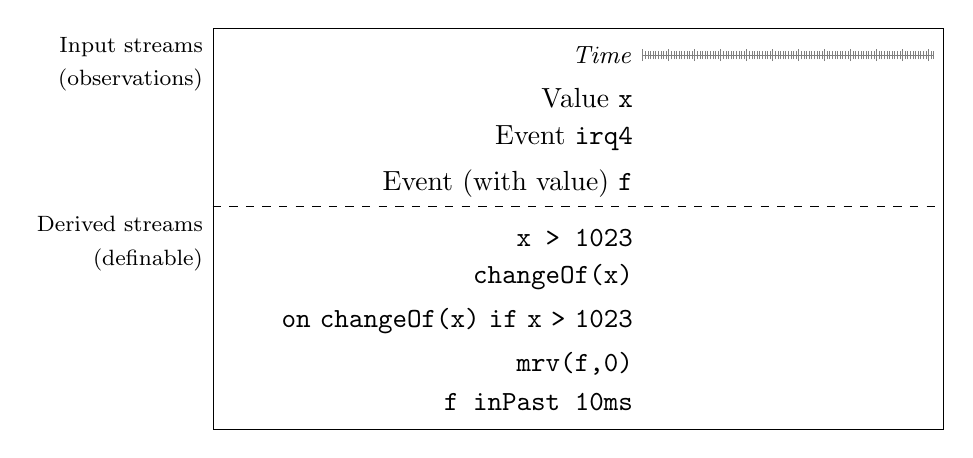
\begin{tikzpicture}

\matrix[column sep = 0.5em, draw] (m) {
  \node[anchor = east] {\small \textit{\textrm{Time}}}; \& \draw[help lines] (0,-0.05) grid[xstep=0.033] (3.7,0.05);
     \draw[gray] (0,-0.075) grid[xstep=0.33] (3.7,0.075); \\[0.5ex]
  \node[anchor = east] (m-1-2) {Value \texttt{x}}; \& \timing[name=m-2-2] at (0,-0.15) {2D{998}N(x1)2D{42}3D{2012}3D{1280}DD{10}DD{1404}};\\
%
  \node[anchor = east] (m-1-3) {Event \texttt{irq4}};
    \& \timing[name=m-2-3] at (0,-0.15) {ZZZ \n{} Z \n{} ZZZZ \n{} ZZ \n{} ZZZ \n{} Z}; \\
%
  \node[anchor = east] (end-inputs) {Event (with value) \texttt{f}};
    \& \timing[name = end-inputs-2] at (0,-0.15) {Z \n{17} ZZZZZZZ \n{98} Z \n{0} ZZZZ \n{23} Z}; \\[0.5em]
%
     \node[anchor = east] (m-1-5) {\texttt{x > 1023}};
  \& \timing[name=m-2-5] at (0,-0.15) {4L 6H 2L 2H}; \\
%
     \node[anchor = east] (m-1-6) {\texttt{changeOf(x)}};
  \& \timing[name=m-2-6] at (0,-0.15) {2Z \n{} 2Z \n{} 3Z \n{} 3Z \n{} 2Z \n{} 2Z}; \\
%
     \node[anchor = east, text width = 14.5em, align = right] (m-1-7) {
          \texttt{\textbf{on} changeOf(x) \textbf{if} x > 1023}};
  \& \timing[name=m-2-7] at (0,-0.15) {4Z \n{} 3Z \n{} 3Z 2Z \n{} 2Z}; \\
%
     \node[anchor = east] (m-1-8) {\texttt{mrv(f,0)}};
  \& \timing[name=m-2-8] at (0,-0.15) {D{0} 7D{17} D{98} 4D{0} D{23}}; \\
%
     \node[anchor = east] (m-1-9) {\texttt{f inPast 10ms}};
  \& \timing[name=m-2-9] at (0,-0.15) {L 2H 5L 3H 2L H}; \\
%
 };

\path[draw, dashed] (m.west|-end-inputs.south) edge (m.east|-end-inputs.south);

\path (m.north west) node[anchor = north east, align = right]
{\footnotesize{Input streams} \\ \footnotesize{(observations)}};

\path (m.west|-end-inputs.south) node[anchor = north east, align = right] {
  \footnotesize{Derived streams} \\ \footnotesize{(definable)}};

\end{tikzpicture}

  \caption{Visualization of \gls{tessla} stream model, taken from~\cite{Decker2016}}
\label{fig:chap2:sec_tessla:streams}
\end{figure}

The syntax of \gls{tessla} is concise, but can be used to define complex functions and specifications:

\begin{align*}
  spec\ \text{::= } &\textttbf{define } name[\textttbf{:}\ stype]\ \textttbf{:= } texpr |\\
                    & \textttbf{out } texpr |
                    spec\ spec\\
  texpr\ \text{:= } & expr[\textttbf{:}\ type] \\
  expr\ \text{:= }  & name \mid literal \mid name\textttbf{(}texpr(\textttbf{, }texpr)^*\textttbf{)}\\
  type\ \text{:= } & btype \mid stype \\
  stype\ \text{:= } & \textttbf{Signal<}btype\textttbf{>} \mid \textttbf{Events<}btype\textttbf{>}
\end{align*}

One of the main contributions of \gls{tessla} is the syntax which mimics modern programming languages and diverges from more clasical approaches in \gls{rv} that use more formal specification languages typically based on logics or automata.
This is an important step to enable practitioners without a strong theoretical background to adopt \gls{rv} techniques in their workflow.
While \gls{rv} has a lot of mechanisms to express specifications they often lack the ability to be intuitively understood.

There are many specification languages like \gls{ltl}~\citep{Pnueli77}, \gls{rltl}~\citep{Leucker2007}, \gls{ctl}~\citep{Clarke82} and many others that are geared heavily toward scientific work and theoretic reasoning.
When introducing new concepts, like realtime, this trend keeps up and formalism like \gls{tltl} from~\cite{Raskin1997}, \gls{stl} from~\cite{Maler2004} and \gls{mtl} from~\cite{Koymans1990} provide theoretical foundations to reason about realtime properties but formulas using these logics are even harder to understand than their non realtime counterparts.

One approach to make \gls{rv} more usage friendly is \gls{salt} presented in~\cite{Bauer2006} which acts as a frontend language to the more formal specification languages and can be translated into them.
\Gls{salt} unifies many different mechanisms, like specification patterns, nested scopes, exceptions, regular expressions and realtime.
\Cref{listing:salt_example} shows an example specification in \gls{salt} taken and adapted from~\cite{Dwyer1999} which specifies that on all three floors in a building, calling the elevator at floor \(\mathit{i}\) implies that it may pass at most two times at that floor without opening its doors, and that it must finally open its doors at that floor within 60 seconds.

\begin{lstlisting}[float,breaklines=true,label=listing:salt_example,caption={[Example \gls{salt} specification with realtime operators]An example specification in the \gls{salt} language taken from \cite{Bauer2006} defining behaviour of an elevator.}]
define max_twice_at_floor_before_open(i) := always (occurring[<=2] atfloor_$i$ between inclusive optional call_$i$ , exclusive optional open_$i$)
define max_60s_before_open(i) := always (call_$i$ implies eventually timed[<=60.0] open_$i$)
assert allof enumerate[1..3] as floor in max_twice_at_floor_before_open(floor) and max_60s_before_open(floor)
\end{lstlisting}

This specification shows, how \gls{salt} specifications are more intuitively understandable than logic formulas, for example by allowing to split the formula in multiple parts and assign meaningful identifiers to subformulas.

\Gls{tessla} and the runtime implemented in this thesis aim to combine many of the aspects that were presented in this Chapter: An understandable specification language like \gls{salt} that is able to express realtime properties, using streams of data as a central element like \gls{lola}, incorporate techniques from \gls{cep} like BeepBeep, and distribute the montitoring to many processors using Erlang and the actor model as shown in \cite{Attard2016}.

\section{Trace Data}
\label{sec:related:traces}

As in \gls{rv} we talk about monitoring of properties over traces, another important aspect is how traces can be extracted from a running program.
Many \gls{rv} tools solve this problem by using a technique called \emph{interweaving}: The code of the monitored program is changed in a way that the monitor becomes part of it, therefore the monitor becomes part of the program and has explicit access to the state of the running system.
Examples for this approach are AspectJ~\cite{Kiczales2001} and DiSL~\cite{Marek2012} for Java, and \gls{rmor}~\cite{Havelund2008} and \gls{rithm}~\cite{Navabpour2013} for C.
This approach is not feasible for the goals of the \gls{tessla} runtime, because we seek the portabilty that enables users to monitor multiple kinds of systems.

Therefore we are looking for ways to manipulate programs in a general way to emit trace data.

As a first step we seeked other projects to extract traces of data that can be used to evaluate the implemented runtime.
While there are many benchmarks available to test monitoring tools we were not able to find any that satisfied all of the characteristics that are needed for an evaluation of \gls{tessla}.
The next sections lists some of the benchmarks and evaluation tools that were surveyed and concludes with a tool that enabled the generation of suitable trace data.

\subsection{General Benchmarks for \glsentryname{rv} Tools}

The field of \gls{rv} lacks a common specification language and can be expanded to a wide variety of different properties to verify.
Therefore it is no surprise that there is no common benchmark that is applicable to all tools.
Nonetheless some benchmarks are occasionally used to compare the expressiveness of a new \gls{rv} tool.

The DaCapo benchmark~\citep{Blackburn2006} was introduced as a general purpose benchmark for the Java language.
It turned out that it can be used to benchmark monitor implementations and trace collection tools~\citep{Wu2016,Chen2007,Marek2012}.
Since Java was not the target architecture of our runtime the DeCapo benchmark was not used for the evaluation in this thesis.

The works in~\cite{Dwyer1999} can be seen as a benchmark for the expressiveness of a specification language.
It categorizes commonly monitored porperties into so called patterns like \emph{precedence}, \emph{absence} and \emph{response}.
While it would be valuable to test \gls{tessla} and the implemented runtimes against these patterns this would be a two step process.
First each pattern would have to be checked, if and how it could be expressed as a \gls{tessla} specification.
As a second step, if the pattern can be expressed, test trace data would have to be generated and only then the runtime could be evaluated using that pattern.
Since this thesis does not work on the \gls{tessla} language definition but only on the runtime we decided not to pursue this gial.

Another interesting project for evaluation of offline monitoring tools is TraceBench presented in~\cite{Zhou2014}.
TraceBench is a big set of traces collected from a distributed system running \gls{hdfs}.
During the collection errors of different categories were deliberately introduced, like network timeouts or data corruption.
The generated traces are organized in a hierarchy: if an event is produced as the effect of another event, for example a function call that leads to another function call, the second event is a child of the first.
Furthermore the traces contain the beginning and end of each event as a timestamp, making the traces suitable for \gls{tessla}.
Unfortunately it seems that the generated trace data has a problem: since events are produced in a distributed system the timestamps are faulty, for example some events started before their parent event.
Furthermore \gls{tessla} doesn't have a mechanism to express nested events as of now, meaning the traces would need to be manipulated before they could be used.

As a final benchmark we evaluated the \gls{crv}~\citep{Reger2016}.
\Gls{crv} has collected a set of benchmarks especially developed for the usage in monitoring algorithms.
It consists of three tracks: Java, C and offline.
While the C and offline track would have been very interesting the benchmarks don't contain any realtime properties.
Since the realtime fragment is an important part of \gls{tessla} we decided that the benchmark wasn't appropriate either.

\subsection{Tools to Generate Traces}

Since no suitable benchmark could be found the next step was to search for a tool that can be used to generate apropriate traces from programs during execution.
These tools can be categorized into static and dynamic instrumentation tools: static tools transform the source code of a program during compilation to include logging statements, dynamic ones only work at runtime and are not involved in the compilation process.

\subsection{CIL}

\Gls{cil} \cite{Necula2002} is a tool to write source-to-source transformations for C programs, therefore it is a static instrumentation tool.
\Gls{cil} implements ``a highly-structured clean subset of C'' in the OCaml language.
\Gls{cil} transforms a C program into an intermediate representation in OCaml.
\Gls{cil} will then apply transformations that are supplied by the programmer to the intermediate representation.
When all transformations are applied the program is written back as a normal C program.

Since \gls{cil} is able to represent the complete C90 standard and also extensions that are commonly used like the ones from GNU C, this tool can be used to write an instrumentation pass for the use case of trace generation.
The main reason that \gls{cil} was not used is that \gls{cil} only supports C and in this thesis we seek a tool that could be used on a variety of programming languages.

\subsection{Google XRay}

Google XRay~\cite{Berris2016} is a function call tracing system for C and \CC.
It is mainly a static instrumentation tool but has some aspects of a dynamic tool.
While XRay requires the orginal source code to be instrumented, the tracing functionality can be turned off at runtime which minimizes overhead.
XRay works by inserting a series of no-ops after function entry points and before return points.
At runtime a library that is part of XRay can then patch these no-ops with instructions to call a log function if tracing is enabled.
This rather complex mechanism is chosen to enable a minimal overhead which was a main requirement for the development of XRay.

XRay is at the moment implemented as a set of patches onto \gls{gcc} but is planned to be migrated to \gls{llvm}.
In typical usage scenarios XRay leads to an overhead of around 20\% to 40\%.

While XRay looks like a promising all-in-one solution to trace collection it only supports the instrumentation of function entrys and exits.
For our instrumentation we wanted to explore the possibility to also trace other events and maybe even allow to attach conditions when an event is actually logged.
As an example consider logging an event whenever a variable is assigned more than once in a single function call.

\subsection{DTrace}

\Cite{Cantrill2004} presents DTrace, a ``facility for dynamic instrumentation of production systems''.
DTrace relies on support from the Kernel of the operating system and does require specific compilation settings for some instrumentations.
DTrace includes a language to specify instrumentations called D.

To use DTrace one has to specify \emph{probes} in the D language.
A \emph{probe} consists of probe descriptions, a predicate and action statements.
The probe descriptions specifies the kind of instrumentation it provides and the modules and functions the probe should be applied to.
The predicate can be used to skip the invocation of the probe if certain conditions are not met.
Action statements contain code that is executed hwen the probe is called.

\Cref{listing:dtrace_spec} shows a DTrace specification with two probes.
The first probe is invoked everytime the instrumetned program calls the \lstinline{read} function provided by the operating system and assigns the current timestamp to a variable.
The second probe is invoked everytime the \lstinline{read} function returns and logs the time used by the \lstinline{read} function before returning.
The predicate of the second probe checks if the variable \lstinline{t} has been assigned.

\begin{lstlisting}[showstringspaces=false,language=C,float,label=listing:dtrace_spec, caption={A DTrace specification in the D language specifying two probes}]
syscall::read:entry {
  self->t = timestamp;
}

syscall::read:return
/self->t/ {
  printf("%d/%d spent %d nsecs in read\n",
    pid, tid, timestamp - self->t);
}
\end{lstlisting}

DTrace offers a variety of instrumentation types, called \emph{providers} in DTrace, \lstinline{syscall} from the previous example being one of them.
Interesting for our research is the \emph{pid} provider which enables the instrumentation of arbitrary instructions in a specified process.
The \emph{pid} provider can be used to log function entrys and exits of every function in a program.

\Cite{Rosenberg2016} builds upon DTrace to build a \gls{rv} framework.
It produces automaton based monitors in the D language from specifications written in \gls{ltl}.
To do so it connects atomic propositions of the formula with observable events that are represented as probes in DTrace.
Whenever a probe is invoked it updates the state of the automaton as specified with the action statements of that probe.

\subsection{LLVM}
\label{sec:related:traces:llvm}

\Gls{llvm}~\cite{Lattner2004} is a compiler framework that allows program analysis and transformation.
The compilation process of \gls{llvm} is seperated into three parts: a front-end, a middle-end and a back-end.
A front-end is responsible for translating a source language, for example C or \CC, into \gls{llvm} \gls{ir}, a strongly typed \gls{risc} instruction set which is independent from the target platform.
The middle-end performs source-to-source transformations on the \gls{ir} that can perform analysis or optimizations.
Such transformations are called \emph{compiler passes} and are independent of the source language.
The back-end is then used to transform the \gls{ir} into native machine code for the target platform.

The \emph{compiler pass} on top of \gls{ir} provides a good abstraction as a base for an instrumentation to generate traces.
Since a pass works on \gls{ir} and not on the source language itself the instrumentation can be used for every language that has an \gls{llvm} front-end.
At the time of writing there is a large collection of such frontends for many languages, including C, \CC, Objective-C, Swift, Haskell, Ruby and many more\footnote{\url{http://llvm.org/ProjectsWithLLVM/}}.

Furthermore a compiler pass can work on all parts of a program: whole modules (think classes in C), function definitions, variable reads and writes, memory allocation and others.
The building block of \gls{ir} programs in \gls{llvm} are the so called \emph{instructions}\footnote{\url{http://llvm.org/docs/doxygen/html/classllvm_1_1Instruction.html}}.
Each statement from a source language is represented as such an instruction.
A \emph{compiler pass} is able to examine instructions, change or reorder them and generate new instructions and insert them appropriately.

Due to the great flexibility that a \emph{compiler pass} offers we chose this approach for the instrumentation pass.
The implementation details can be seen in \Cref{sec:implementation:instrumentation}.

 % INCLUDE: related work
% !TEX root = ../thesis.tex
%
\chapter{System}
\label{sec:system}

TODO: This will become Implementation details chapter, move unrelated stuff to Related work

Besides the theoretical basics presented in \cref{sec:related} the \gls{tessla} runtime of this thesis is built upon a number of technologies.
To better understand decisions made during the implementation this chapter will give an overview of them and show why they were choosen.

As already mentioned, the implemented runtime itself is independent of the way traces are generated.
Therefore we will not only look at building blocks for the runtime itself but also examine related projects which can be used to obtain traces, which then can be monitored by the runtime.
Because the format of the traces can differ heavily, depending on how and why they were collected, they are not only used to test the runtime but also to determine how it can consume them.

\section{\glsentryname{tessla} Runtime}
\label{sec:system:runtime}

The runtime to evaluate specifications is implemented in the programming language Elixir, which itself is built on top of Erlang.
To understand why this plattform was choosen we will look at the Erlang ecosystem in the next section.

\subsection{Erlang and Elixir}
\label{sec:system:eval_engine:erlang_elixir}
\todo{BEAM, Actors/Thread, multiplattform (nerves project)}
\subsection{Implementation}
\todo{Timing model: reason why events have to carry timestamps in contrast to interweaved monitors}

\section{Trace Data}
\label{sec:system:traces}

Problem: Many traces don't carry timestamp (see DeCapo, CRV 15)

\url{http://lttng.org}
\url{http://diamon.org/ctf/}
\url{https://github.com/efficios/barectf}
\subsection{Debie}
\subsection{TraceBench}
\subsection{Aspect oriented programming}
\subsection{CIL}
\subsection{Google XRay}
\subsection{GCC instrument functions}
\subsection{Sampling}
\subsection{LLVM/clang AST matchers}
	% INCLUDE: system
% % !TEX root = ../thesis-example.tex
\chapter{Concepts}
\label{sec:concepts}

In this chapter different ways to evaluate \gls{tessla} specifications are given and their equivalence is shown.
To do so in Section~\ref{sec:concepts:defs} building blocks for evaluation approaches are defined, which are then used in later sections to define behaviour of them and show their equivalence.

\section{Definitions}
\label{sec:concepts:defs}

While the \gls{tessla} specification itself defines a set of semantics, for this thesis we will slightly alter some of it and add some new definitions based on them.
This is necessary to reason about the specifics how the evaluation engine is built (Note that \gls{tessla} doesn't define an operational semantic, therefore we will define our own) and how it behaves.

\subsection{Time}
\label{sec:concepts:defs:time}

\gls{tessla} has a model of continuous time, where timestamps \(t \in \mathbb{T} \) are used to represent a certain point in time and \(\mathbb{T}\) has to be isomorphic to \(\mathbb{R}\).

\subsection{Transducers}
\label{sec:concepts:defs:transducers}

Fundamentally \gls{tessla} is a special kind of a transducer.
Therefore in this section we will define a model of transducers which can be used to reason about the evaluation of a \gls{tessla} specification.

A transducer is a system, which consumes an input and produces an output.
Let \(\Phi, \Gamma\) be two alphabets and \(\epsilon\) the empty word.

\begin{definition}[name = Transducer]\label{def:transducer}
  A transducer \(t\) is a relation \(t \subseteq \Phi^* \times \Gamma^*\), \(\Phi\) is called the input alphabet, \(\Gamma\) the output alphabet.
\end{definition}

\gls{tessla} specifications are deterministic for any input, meaning they should produce the same output for the same input.

\begin{definition}[name = Deterministic Transducer]\label{def:deterministic_transducer}
  A deterministic transducer relates each input to at most one output.
\end{definition}

\begin{exmp}[name = Deterministic and Nondeterministic Transducers]
  \(t_d = \{(a,1),(b,2),(ab,12),(ba,21)\}\) is a deterministic transducer, \(t_{nd} = \{(a,1),(a,2)\}\) is nondeterministic, because it relates \(a\) to \(1\) and \(2\).
\end{exmp}

Transducers can furthermore be categorized as synchronous, asynchronous, causal and clairvoyant transducers:
synchronosity is a property over the behaviour of a transducer when it's consuming input per element.
If it is synchronous, it will produce an output element for each input element.

\begin{definition}[name = Synchronous Transducer]\label{def:synchronous_transducer}
Let \(\vec{\imath} \in \Phi^*, i \in \Phi, \vec{o} \in \Gamma^*, o \in \Gamma\).
  A transducer \(t\) is called synchronous, when it satisfies, that:
  if \( (\vec{\imath}\circ i,\vec{o}\circ o) \in t\)
  then \( (\vec{\imath}, \vec{o}) \in t \)
\end{definition}

An asynchronous transducer can produce zero, one or many outputs for each input it consumes.

\begin{definition}[name = Asynchronous Transducer]\label{def:asynchronous_transducer}
  Let \(\vec{\imath}\in \Phi^*, i \in \Phi,\vec{o} \in \Gamma^*\).
  A transducer \(t\) is called asynchronous when it satisfies the formula:
  if \((\vec{\imath}\circ i, \vec{o}) \in t \)
  then \(\exists \vec{o'},\vec{o''} \in \Gamma^*\text{ so that } \vec{o} = \vec{o'}\circ\vec{o''} \text{ and } (\vec{\imath},\vec{o'}) \in t \)
\end{definition}

\begin{exmp}[name = Synchronous and Asynchronous Transducers]
  \(t_s = \{(a,1),(b,2),(ab,12),(ba,21)\}\) is a synchronous transducer, \(t_{as} = \{(a,\epsilon),(ab,12)\}\) is asynchronous.
\end{exmp}

A causal transducer is one, where the output depends only on consumed inputs and not on future inputs:

\begin{definition}[name = Causal and Clairvoyant Transducers]\label{def:causal_transducer}
  A transducer \(t\) is called causal, when it satiesfies, that:
  if \((\vec{\imath},\vec{o}) \in t \)
  then \( \forall \vec{\imath'} \in \Phi^* \text{ with } (\vec{\imath} \circ \vec{\imath'}, \vec{o'}) \in t \)
  it holds, that \( \vec{o} \sqsubseteq \vec{o'} \)

  A transducer that isn't casual is called \emph{clairvoyant}.
\end{definition}


\begin{exmp}[name = Causal and Clairvoyant Transducers]
  \(t_{cl} = \{(a,1),(b,2),(ab,12),(ba,21)\}\) is a causal transducer, because each output only depends on the inputs seen upto that point, \(t_{cl} = \{(a,1),(ab,22),(aa,11)\}\) is clairvoyant, because the output when the letter \(a\) is seen depends on the next input.
\end{exmp}

When talking about transducers, it is interesting to know if two transducers are \emph{equivalent}.
There are multiple possible definitions for equivalence of transducers, we will look at two, which are interesting for this thesis.
In the following \(\sigma_i\) is used to get the element at position \(i\) and \(\sigma_{[i,j]}\) to get the infix of \(\sigma\) which starts at position \(i\) and ends at position \(j\) (With \(0\) as the index of the first element).

\begin{definition}[name = Asynchronous equivalence of Transducers]\label{def:async_equivalence_transducer}
  Let \(t_1, t_2\) be two asynchronous transducers from \(\Phi^*\) to \(\Gamma^*\).
  They are called \emph{asynchronous equivalent}, written \(t_1 \equiv_a t_2\), if they satisfy: \\
  \(\forall \sigma \in \Phi^*\):
  \begin{itemize}
    \item \(\forall (\sigma_{[0,k]}, \vec{o}) \in t_1\): \(\exists k' \geq k \text{ with } (\sigma_{[0,k']}, \vec{o'}) \in t_2\) and \(\vec{o} \sqsubseteq \vec{o'}\)
    \item and \(\forall (\sigma_{[0,k]}, \vec{o}) \in t_2\): \(\exists k' \geq k \text{ with } (\sigma_{[0,k']}, \vec{o'}) \in t_1\) and \(\vec{o} \sqsubseteq \vec{o'}\)
  \end{itemize}
\end{definition}

\begin{lemma}[name=Asynchronous equivalence is an equivalence Relationship]\label{lemma:async_equivalence_is_equivalence_relationship}
  Asynchronous equivalence is symmetric, reflexive and transitive.
\end{lemma}
\begin{proof}$ $\newline
  \begin{itemize}
    \item Symmetry: trivial, since the second part of the definition is requiring it.
    \item Reflexivity: Also trivial, for \((\sigma_{[0,k]}, \vec{o})\) select \(k' = k\).
    \item Transitivity:
      \begin{itemize}
        \item Let \(t_1 \equiv_a t_2\), \(t_2 \equiv_a t_3\).
        \item First case:
          \begin{align*}
            &\text{Since } t_1 \equiv_a t_2:\ \forall (\sigma_{[0,k_1]}, \vec{o_1}) \in t_1: \\
            &\hspace{2em} \exists k_2\ \text{such, that } (\sigma_{[0,k_2]}, \vec{o_2}) \in t_2\ \text{with } \vec{o_1} \sqsubseteq \vec{o_2} \\
            &\hspace{2em} \text{and since } t_2 \equiv_a t_3 \\
            &\hspace{4em} \exists k_3\ \text{such, that } (\sigma_{[0,k_3]}, \vec{o_3}) \in t_3\ \text{with } \vec{o_2} \sqsubseteq \vec{o_3}\\
            &\hspace{4em} \text{With } \vec{o_1} \sqsubseteq \vec{o_2} \sqsubseteq \vec{o_3}\ \text{it follows, that } t_1 \equiv_a t_3
          \end{align*}
        \item The second case works the same, just change \(t_1\) and \(t_3\).
      \end{itemize}
  \end{itemize}
\end{proof}

\begin{exmp}[name = Asynchronous equivalence of Transducers]
  Let \(\Phi = \{a\}, \Gamma = \{1\}\) and \\
  \begin{align*}
    &t_1 = \{&&(a,\epsilon),  &&(aa,\epsilon),  &&(aaa,111)   &\} \\
    &t_2 = \{&&(a,1),         &&(aa,1),         &&(aaa,111)   &\} \\
    &t_3 = \{&&(a,\epsilon),  &&(aa,1),         &&(aaa,11)    &\}\\
  \end{align*}
  All three transducers are asynchronous and causal.
  Let's see which ones are asynchronous equivalent:

  \(t_1 \stackrel{?}{\equiv}_a t_2\)
  \begin{align*}
    &(a,\epsilon)  &&\in t_1, k = 1 &\rightarrow k' = 1, &(a,1)     \in t_2, &\epsilon  &\sqsubseteq 1 \\
    &(aa,\epsilon) &&\in t_1, k = 2 &\rightarrow k' = 2, &(aa,1)    \in t_2, &\epsilon  &\sqsubseteq 1 \\
    &(aaa,111)     &&\in t_1, k = 3 &\rightarrow k' = 3, &(aaa,111) \in t_2, &111       &\sqsubseteq 111 \\
    &(a,1)         &&\in t_2, k = 1 &\rightarrow k' = 3, &(aaa,111) \in t_1, &1         &\sqsubseteq 111 \\
    &(aa,1)        &&\in t_2, k = 2 &\rightarrow k' = 3, &(aaa,111) \in t_1, &1         &\sqsubseteq 111 \\
    &(aaa,111)     &&\in t_2, k = 3 &\rightarrow k' = 3, &(aaa,111) \in t_1, &111       &\sqsubseteq 111 \\
  \end{align*}
  \(\Rightarrow t_1 \equiv_a t_2\)

  \(t_1 \stackrel{?}{\equiv}_a t_3\)
  \begin{align*}
    &(aaa,111)     \in t_1, k = 3 \rightarrow \not\exists k'
  \end{align*}
  \(\Rightarrow t_1 \not\equiv_a t_3\)

  Because of Lemma~\ref{lemma:async_equivalence_is_equivalence_relationship} \(\Rightarrow t_2 \not\equiv_a t_3\).

\end{exmp}

\subsection{Timed Transducers}\label{sec:concepts:def:timed_transducer}

For the second kind of equivalence we need to introduce \emph{timed sequences} and \emph{timed transducers}.
Let \(\mathbb{T}\) be a timing model that is isomorphic to \(\mathbb{R}\).
For the examples we will use \(\mathbb{R}\) for \(\mathbb{T}\).

\begin{definition}[name = Timed Sequence]\label{def:timed_sequence}
  A sequence is called timed, if every element of it is associated with a timestamp: \(\sigma \in {(\Gamma\times\mathbb{T})}^*\).
  For bravety a timed sequence can be written with the timestamps as the index of the elements: \(\sigma = e_0e_{0.5}e_1 \).\\
  The function
  \[\mathit{timed: } {(\Gamma \times \mathbb{T})}^* \rightarrow {(\Gamma \times \mathbb{T})}^* \]
  reorders a timed sequence \(\sigma\) by its timestamps, such that:
  \[ \forall i,j \in \mathbb{N}:\text{ if } i < j \text{ then } t_i < t_j \text{ with } (o_i, t_i) = \sigma_i \text{ and } (o_j, t_j) = \sigma_j \]
  The function
  \[\mathit{upto: } \mathbb{T} \times {(\Gamma\times\mathbb{T})}^* \rightarrow {(\Gamma\times\mathbb{T})}^*\]
  removes all elements from a timed sequence, that have a timestamp bigger than the first argument.\\
  The function
  \[\mathit{maxTime: } {(\Gamma\times\mathbb{T})}^* \rightarrow \mathbb{T} \]
  returns the biggest Timestamp in a timed sequence.
\end{definition}

\begin{exmp}[name=Functions on timed Sequences]
Let \(\sigma = a_1a_{0.5}a_{1.5}a_0\).\\
  Then is
    \begin{align*}
      &\mathit{timed} (\sigma) = a_0a_{0.5}a_1a_{1.5}\ \\
      &\mathit{upto} (1.3,\sigma) = a_1a_{0.5}a_0 \\
      &\mathit{maxTime} (\sigma) = 1.5
    \end{align*}
\end{exmp}

\begin{definition}[name = Monotonicity of Timed Sequences]\label{def:monotonicity_timed_sequences}
  A timed sequence \(\sigma\) with alphabet \(\Phi\) is called monotonic,
  if \( \mathit{timed}(\sigma) = \sigma\)
\end{definition}

\begin{definition}[name = Timed Transducer]\label{def:timed_transducer}
  A timed transducer \(t\) with input alphabet \(\Phi\) and output alphabet \(\Gamma\) works on monotonic, timed sequences as inputs and has timed sequences as outputs:
  \[t \subset {\left(\Phi \times \mathbb{T}\right)}^* \times {\left(\Gamma \times \mathbb{T}\right)}^*\]
  % Furthermore a timed transducer has to be causal and asynchronous.
\end{definition}

\begin{exmp}[name=Timed Transducers]
  Let \(\Phi = \{a\}, \Gamma = \{b\}\).\\
  \(t_{tsc} = \{(a_0, b_0),(a_0a_1, b_0b_1)\}\) is a timed, causal and synchronous transducer.\\
  \(t_{tac} = \{(a_0, \epsilon),(a_0a_1, b_0b_1)\}\) is a timed, causal and asynchronous transducer.
\end{exmp}


For later theoretic work we have to restrict timed transducers:

\begin{definition}[name = Boundedness of Timed Transducers]\label{def:boundedness_timed_transducer}
  A timed transducer \(t\) with input alphabet \(\Phi\) and output alphabet \(\Gamma\) is called bounded, if it satisfies:
  \begin{align*}
    &\forall \sigma \in {(\Phi \times \mathbb{T})}^*:\\
    &\hspace{2em}\text{if } (\sigma_{[0,k]}, \vec{o}) \in t\\
    &\hspace{2em}\text{then }\exists k' > k\ \text{with}\\
    &\hspace{4em}(\sigma_{[0,k']}, \vec{o} \circ \vec{o'}) \in t\\
    &\hspace{4em}\text{and} \forall k'' > k'\ \text{with } (\sigma_{[0,k'']}, \vec{o}\circ\vec{o'}\circ\vec{o''}) \in t\ \text{it holds, that}\\
    &\hspace{6em}\mathit{upto}(\mathit{maxTime}(\vec{o}), \mathit{timed}(\vec{o}\circ\vec{o'})) = \mathit{upto}(\mathit{maxTime}(\vec{o}), \mathit{timed}(\vec{o}\circ\vec{o'}\circ\vec{o''}))
  \end{align*}
\end{definition}

Based on the definitions we can define an equivalence relationship on bounded timed transducers:

\begin{definition}[name = Observational Equivalence]\label{def:observational_equivalence}
  Let \(t_1, t_2\) be two bounded timed transducers with input alphabet \(\Phi\) and output alphabet \(\Gamma\).
  They are called \emph{observational equivalent}, written \(t_1 \equiv_o t_2\), if they satisfy:
  \begin{align*}
    &\forall \sigma \in {(\Phi\times\mathbb{T})}^*:\\
    &\hspace{2em}\forall (\sigma_{[0,k]}, \vec{o}) \in t_1: \exists k', k'' \geq k\ \text{such that}\\
    &\hspace{4em}(\sigma_{[0,k']}, \vec{o} \circ \vec{o'}) \in t_1\\
    &\hspace{4em}\text{and } (\sigma_{[0,k'']}, \vec{o_2}) \in t_2\\
    &\hspace{4em}\text{and } \mathit{timed}(\mathit{upto}(\mathit{maxTime}(\vec{o}),\vec{o} \circ \vec{o'} )) = \mathit{timed}(\mathit{upto}(\mathit{maxTime}(\vec{o}),\vec{o_2}))
  \end{align*}
  and the same for switched \(t_1, t_2\).
\end{definition}

\begin{lemma}[name=Observational Equivalence is an Equivalence Relationship for Bounded Transducers]\label{lemma:observational_equivalence_equivalence_relationship}
  \(\equiv_o\) is symmetric, reflexive and transitive for bounded timed transducers.
\end{lemma}
\begin{proof}$ $\newline
  Let \(t_1, t_2, t_3\) be bounded timed transducers.
  \begin{itemize}
    \item Symmetry: By definition.
    \item Reflexivity: For \((\sigma_{[0,k]}, \vec{o})\) select \(k' = k''\) as the k, for which the transducer is bounded for that input.
    \item Transitivity:
      \begin{itemize}
        \item Let \(t_1 \equiv_o t_2\), \(t_2 \equiv_o t_3\).
        \item First case:
          \begin{align*}
            &\text{Since } t_1 \equiv_o t_2:\ \forall (\sigma_{[0,k_1]}, \vec{o_1}) \in t_1: \\
            &\hspace{2em} \exists k_1', k_2 > k_1\ \text{with } (\sigma_{[0,k_1']}, \vec{o_1}\circ\vec{o_1'}) \in t_1\ \text{and } (\sigma_{[0,k_2]}, \vec{o_2}) \in t_2 \\
            &\hspace{4em} \text{with } \mathit{timed}(\mathit{upto}(\mathit{maxTime}(\vec{o_1}),\vec{o_1} \circ \vec{o_1'} )) \\
            &\hspace{8em} = \mathit{timed}(\mathit{upto}(\mathit{maxTime}(\vec{o_1}),\vec{o_2})) & (\star)\\
            &\hspace{2em} \text{and since } t_2 \equiv_o t_3: \exists k_2', k_3 > k_2\ \text{with } (\sigma_{[0,k_2']}, \vec{o_2}\circ\vec{o_2'}) \in t_2 \\
            &\hspace{4em} \text{and } (\sigma_{[0,k_3]}, \vec{o_3}) \in t_3 \\
            &\hspace{6em} \text{with } \mathit{timed}(\mathit{upto}(\mathit{maxTime}(\vec{o_2}),\vec{o_2} \circ \vec{o_2'} )) \\
            &\hspace{10em} = \mathit{timed}(\mathit{upto}(\mathit{maxTime}(\vec{o_2}),\vec{o_3})) & (\star\star)\\
            &\hspace{2em} \mathit{maxTime}(\vec{o_1})\ \text{has to be smaller then}\mathit{maxTime}(\vec{o_2}) \\
            &\hspace{4em} \text{else } (\star)\ \text{couldn't hold, therefore, combined with boundedness and }(\star\star): \\
            &\hspace{4em} \mathit{timed}(\mathit{upto}(\mathit{maxTime}(\vec{o_1}),\vec{o_2} )) \\
            &\hspace{8em} = \mathit{timed}(\mathit{upto}(\mathit{maxTime}(\vec{o_1}),\vec{o_3})) \\
            &\text{which concludes }\mathit{timed}(\mathit{upto}(\mathit{maxTime}(\vec{o_1}),\vec{o_1} \circ \vec{o_1'} ))\\
            &\hspace{4em} = \mathit{timed}(\mathit{upto}(\mathit{maxTime}(\vec{o_1}),\vec{o_3}))
          \end{align*}
        \item The second case works the same, just switch \(t_1\) and \(t_3\).
      \end{itemize}
  \end{itemize}
\end{proof}


\begin{exmp}[name=Observational Equivalence]\label{exmp:observational_equivalence}
  Let
  \begin{align*}
    &t_1 = \{&&(a_0, \epsilon),   &&(a_0a_1, b_1),      &&(a_0a_1a_2, b_1b_2b_0)  &\} \\
    &t_2 = \{&&(a_0, \epsilon),   &&(a_0a_1, \epsilon), &&(a_0a_1a_2, b_2b_1b_0)  &\} \\
    &t_3 = \{&&(a_0, b_0),        &&(a_0a_1, b_0),      &&(a_0a_1a_2, b_2b_1)     &\}
  \end{align*}
  All three are causal, asynchronous timed transducers.

  Let's see which ones are observational equivalent:

  \(t_1 \stackrel{?}{\equiv}_o t_2\)
  \begin{itemize}[label={}]
    \item \((a_0, \epsilon)             \in t_1, k = 1, \mathit{maxTime}(\epsilon) = 0\)
      \begin{itemize}[label={}]
        \item \(\rightarrow k' = 1, (a_0, \epsilon)     \in t_1\)
        \item \(\rightarrow k'' = 1, (a_0, \epsilon)     \in t_2\)
      \end{itemize}
    \item \((a_0a_1, b_1)               \in t_1, k = 2, \mathit{maxTime}(b_1) = 1\)
      \begin{itemize}[label={}]
        \item \(\rightarrow k' = 3, (a_0a_1a_2, b_1b_2b_0)    \in t_1\)
        \item \(\rightarrow k'' = 3, (a_0a_1a_2, b_2b_1b_0)    \in t_2\)
        \item \(\mathit{timed}(\mathit{upto}(1, b_1b_2b_0)) = b_0b_1 = \mathit{timed}(\mathit{upto}(1, b_2b_1b_0))\)
      \end{itemize}
    \item \((a_0a_1a_2, b_1b_2b_0)               \in t_1, k = 3, \mathit{maxTime}(b_1b_2b_0) = 2\)
      \begin{itemize}[label={}]
        \item \(\rightarrow k' = 3, (a_0a_1a_2, b_1b_2b_0)    \in t_1\)
        \item \(\rightarrow k'' = 3, (a_0a_1a_2, b_2b_1b_0)    \in t_2\)
        \item \(\mathit{timed}(\mathit{upto}(2, b_1b_2b_0)) = b_0b_1b_2 = \mathit{timed}(\mathit{upto}(2, b_2b_1b_0))\)
      \end{itemize}
    \item \((a_0, \epsilon)               \in t_2, k = 1, \mathit{maxTime}(\epsilon) = 0\)
      \begin{itemize}[label={}]
        \item \(\rightarrow k' = 1, (a_0, \epsilon)     \in t_2\)
        \item \(\rightarrow k'' = 1, (a_0, \epsilon)     \in t_1\)
      \end{itemize}
    \item \((a_0a_1, \epsilon)            \in t_2, k = 2, \mathit{maxTime}(epsilon) = 0\)
      \begin{itemize}[label={}]
        \item \(\rightarrow k' = 2, (a_0a_1, \epsilon)    \in t_2\)
        \item \(\rightarrow k'' = 2, (a_0a_1, b_1)    \in t_1\)
        \item \(\mathit{timed}(\mathit{upto}(0, \epsilon)) = \epsilon = \mathit{timed}(\mathit{upto}(0, b_1))\)
      \end{itemize}
    \item \((a_0a_1a_2, b_2b_1b_0)        \in t_2, k = 3, \mathit{maxTime}(b_2b_1b_0) = 2\)
      \begin{itemize}[label={}]
        \item \(\rightarrow k' = 3, (a_0a_1a_2, b_2b_1b_0)    \in t_2\)
        \item \(\rightarrow k'' = 3, (a_0a_1a_2, b_1b_2b_0)    \in t_1\)
        \item \(\mathit{timed}(\mathit{upto}(2, b_2b_1b_0)) = b_0b_1b_2 = \mathit{timed}(\mathit{upto}(2, b_1b_2b_0))\)
      \end{itemize}
  \end{itemize}
  \(\Rightarrow t_1 \equiv_a t_2\)

  \(t_1 \stackrel{?}{\equiv}_a t_3\)
  \begin{itemize}[label={}]
    \item \((a_0a_1a_2,b_1b_2b_0)      \in t_1, k=3, \mathit{maxTime}(b_1b_2b_0) = 2\)
      \begin{itemize}[label={}]
        \item \(\rightarrow k' = 3, (a_0a_1a_2, b_1b_2b_0)    \in t_1\)
        \item \(\rightarrow \not\exists (\vec{\imath}, \vec{o}) \in t_3\ \text{with } \exists n \in \mathbb{N}: \vec{o}_n = b_0\)
        \item \(\rightarrow \not\exists (\vec{\imath}, \vec{o}) \in t_3\ \text{with } \mathit{timed}(\mathit{upto}(2, b_1b_2b_0)) = b_0b_1b_2 = \mathit{timed}(\mathit{upto}(2,\vec{o}))\)
      \end{itemize}
  \end{itemize}
  \(\Rightarrow t_1 \not\equiv_a t_3\)\\
  If \(t_3\) weren't bounded (and therefore not finite) there would be no way to know, if it was equivalent to \(t_1\), because it could always produce a missing event at a later time.

  Because of Lemma~\ref{lemma:observational_equivalence_equivalence_relationship} \(\Rightarrow t_2 \not\equiv_a t_3\).

\end{exmp}

\subsection{Labeled Timed Transducers}
Maybe necessary, maybe not

\subsection{Events}
\label{sec:concepts:defs:events}

Events are the atomic unit of information that all computations are based on.
There are three types of events: external, output and internal events.

The set of all events is denoted as \(E\).
Each event carries a value, which can be \emph{nothing} or a value of a type (types are formally defined in the \gls{tessla} specification, but aren't important for this thesis), a timestamp and the stream it's perceived on (e.g.\ a function call of a specific function or the name of an output stream).

The value of an event can be queried with the function \(\upsilon\), its timestamp with \(\pi\) and its stream with \(\mathit{stream}\).

\(E_e \subset E\) is the set of all external events, their stream corresponds to a specific trace.
\(E_o \subset E\) is the set of all output events, their stream is specified by an output name of the \gls{tessla} specification.
\(E_n \subset E\) is the set of all internal events.
Internal events are mostly an implementation dmathit{node}il, which denote steps of computation inside the runtime.
The stream of internal events is implicitly given by the node that produces the stream of the event.
Note that \(E_e, E_o, E_n\) are pairwise disjoint and \(E_e \cup E_o \cup E_n = E\).

\subsection{Streams}
\label{sec:concepts:defs:streams}

Streams are a collection of events with specific characteristics.
While events are the atomic unit of information, streams represent the sequence of related events over time.

There are two kind of streams: signals, which carry values at all times, and event\-streams, which only hold values at specific times.
Eventstreams can be described by a sequence of events.
Signals can be described by a sequence of changes, where a change denotes that the value of a signal changed at a specific timestamp.
The only difference between a signal and an eventstreams is that signals always have a value while an eventstream may return \(\bot\) when queried for its value at a specific time, which denotes that no event happened at that time.
Based on the similarity of signals and eventstreams in the following we will mainly reason about eventstreams, but most things can also be applied to signals.

Formally a stream \(\sigma\) can be represented as the product of a sequence of events \(\langle e_1, \dots e_n\rangle\) where \(\pi(e_i) < \pi(e_{i+1}),\ \forall i < n \in \mathbb{N}\) and a value from \(\mathbb{T}\) which marks the progress of the stream and has to be equal or bigger to the timestamp of the last event.
The set of all streams \(\Sigma\) is defined as all possible finite sequences of events \(\Sigma = \{\sigma | \sigma \in E^* \} \times \mathbb{T}\).
An external stream \(\sigma_e\) is a stream consisting only of external events, the set of all external streams is \(\Sigma_e = \{\sigma_e | \sigma_e \in E_e^*\} \times \mathbb{T}\).
Output and internal streams are defined analogous.

To get the event of a stream \(\sigma\) at a timestamp \(t\) it can be queried like a function: \(\sigma(t) = e\) with \(\pi(e) = t \).
When working with signals, the function will return the latest event that happened at or before t while an eventstream may return \(\bot\).
The progress of a stream can be obtained with \(\mathit{progress}(\sigma) = t \in T\).
Internal and output streams can be queried for the node that produced them with \(\mathit{node}(\sigma) = n \in N\).

\subsection{Functions}
\label{sec:concepts:defs:functions}

A \gls{tessla} specification consists of functions over streams.
Functions generate new streams by applying an operation on existing streams.
\gls{tessla} itself defines a syntax to write a specification, a set of types and a standard library of functions, but an implementation is free to choose the functions it supports.

An example function is \(add(S_D,S_D) \rightarrow S_D\): It takes two signals, which have to hold values of some numerical type, and produces a signal which holds values of the same type.
The produced stream can either be assigned to a named identifier (think: a variable) or consumed by another function (function composition).

Functions can be divided into three categories: pure, unpure and timing.
Pure functions, also called stateless, are evaluated only on the values their inputs have at the timestamp they are evaluated, therefore they don't have to \emph{remember} anything about earlier events.
Unpure, or stateful, functions are evaluated over the whole input stream, meaning they can look at all events that happened on its inputs before the time of evaluation and also at all it's previous output events.
E.g.\ a function \emph{eventCount} has to \emph{remember} how many events already happened on it's input stream and increment that counter on every new event.
Timing functions are evaluated not only on the value of events but also on their timestamp and can also manipulate it:
While non timing functions will consume events at a specific timestamp and emit events with that timestamp, timing functions can emit events with a changed timestamp.
In this thesis we will only look at past time functions, meaning functions can only delay timestamps, therefore can't depend on future values.

Timing functions complicate the reasoning about schedules and causality and therefore aren't included in Section~\ref{sec:concepts:behaviour_without_timing}.
In Section~\ref{sec:concepts:behaviour_with_timing} the conclusions of earlier sections will be extended to include timing functions.


\subsection{Nodes}
\label{sec:concepts:defs:nodes}

Nodes are the atomic unit of computation for the evaluation of a \gls{tessla} specification.
A node implements a single function, e.g.:\ there is an \emph{AddNode} which takes two input signals and produces a new signal.
Therefore a node is the concrete implementation of a function in a runtime for \gls{tessla} specifications.
The set of all nodes is called \(N\).
The function of a node \(n \in N\) is written as \(f_n\).

Each node has a set of inputs, which are either external or internal streams, and one output, which is either an internal or an output stream.
Nodes which have at least one external stream as an input are called \emph{sources}.
Nodes have \gls{fifo} queues, provided by the Erlang plattform, which buffer events from the inputs for later computation.
Furthermore they have a timestamp for each input that encodes the progress of that input.
Based on the queues, the timestamps of the inputs and it's function, a node performs its computation in multiple steps:

\begin{enumerate}
  \item Check if one or more new output events can be produced (see Section~\ref{sec:concepts:defs:nodes:processable})
    \begin{itemize}
      \item If so, compute all timestamps, where new events might be computed
      \item Compute the events at the possible timestamps
      \item Remove the used Events for the computation from the input queue
    \end{itemize}
  \item Afterwards check if the progress of the output can be updated
    \begin{itemize}
      \item The progress always is the minimum of the timestamps of all inputs
    \end{itemize}
  \item Add the produced events to the input of all children and update the associated progress to the new one
\end{enumerate}

\subsubsection{Determination of processable Events}
\label{sec:concepts:defs:nodes:processable}

Based on the asynchronous nature of nodes, events from different streams can be received out of order.
Therefore a node cannot compute its output upto a timestamp unless it has the information from all inputs that they did progress to at least that timestamp.

E.g.\ if a node \(c\) is a child of node \(a\) and \(b\), it can receive events from node \(a\) at timestamps \(t_1, t_2, t_3, t_4\) before receiving an event with timestamp \(t_1\) from node \(b\).
When node \(c\) receives the first four events from node \(a\), they will stay buffered on the input queue that represents the stream from node a and the progress for that input will be \(t_4\), while the input queue representing the stream from node b will have no events buffered and a progress of \(0\).
When it receives the first event from node \(b\) it can compute all events upto \(t_1\).
To do so it will compute \emph{change timestamps}: The union of all timestamps where an event occured on any input between the timestamp of the last generated output and the minimal progress of all inputs.
In this case that is only \(t_1\).
Therefore the node will remove the events with timestamp \(t_1\) from both queues and will compute a new event based on them, with a timestamp that is equal to or smaller than \(t_1\), where smaller can only happen if it is a timing node.
Then it will distribute the computed event together with the new progress \(t_1\) to its children.

To see why the computation of change timestamps is necessary lets assume that node \(c\) will receive a new event from node \(b\) with timestamp \(t_4\):
All inputs have progressed to \(t_4\), but on the stream from node \(a\) there are changes between \(t_1\) (where the last output was generated) and \(t_4\), therefore the \emph{change timestamps} are \(t_2, t_3, t_4\) and the node will have to compute its output based on the values of the streams at that timestamps.

\subsection{\glsentryname{tessla} Evaluation Engine}
\label{sec:concepts:def:eval_engine}

Because functions in \gls{tessla} specifications depend on other functions, and these dependencies have to be circle free, the specification can be represented as a \gls{dag}, where the functions are vertices and the relationship between functions are edges.
This is exactly how the \gls{tessla} compiler outputs a specification.
One can now use the \gls{dag} of a \gls{tessla} specification to synthesize a system to evaluate it over inputs:
The vertices of the \gls{dag} become nodes representing the functions and the edges are the input and output streams between the nodes.
We will call this synthesized system an \emph{evaluation engine}.

When fed with inputs (or \emph{traces}) the engine will produce outputs.
The relationship between inputs and outputs that is produced can be seen as a timed transducer.

To evaluate a specification over traces, the evaluation engine has process the events that were traced.
To do so the nodes have to run their computations until no more events are present (or the specification found an error in the trace).
This leads to the question in which order nodes should be scheduled to perform their computation.
While some schedules are simply not rational (think of unfairness and causality), there are many different schedules that are feasible.
It has to be prooven that a chosen schedule produces the correct conclusions for a specification, else the evaluation engine is not valid.

This proof will be carried out for different kinds of schedules in Section~\ref{sec:concepts:equivalence_without_timing}, showing that all of them can be used by an evaluation engine.
For now we can define when to evaluation engines are called equivalent based on the work in Section~\ref{sec:concepts:def:timed_transducer}:

\begin{definition}[name=Equivalence of Evaluation Engines]\label{def:equivalence_eval_engine}
  Two evaluation engines are called equivalent, if their produced relationships between inputs and outputs are observational equivalent.
\end{definition}

Because the possible inputs are infinite we will restrict the definition of equivalence to a specified set of inputs:

\begin{definition}[name=Equivalence of Evaluation Engines for Specified Inputs]\label{def:equivalence_eval_engine_specific_inputs}
  Two evaluation engines are called equivalent for a set of inputs, if the relationship for theese inputs and the produced outputs is observational equivalent.
\end{definition}


\subsection{State and History}
\label{sec:concepts:def:state}

All \gls{tessla} evaluation engines have to hold a state, which encodes information necessary to continue the evaluation, and a history, which encodes what happened on all streams in the evaluation engine.
The state of a whole evaluation engine is made up of the states of its nodes.

Each node has a state, which can hold arbitray information, e.g.\ a counter for a \emph{CountNode}, and its input queues.
Input queues are \gls{fifo} queues, which hold the events produced by predecessors of the node, that weren't consumed yet by the node.

To distinguish between the two types of states, the state of the whole engine is called the \emph{global state} and the state of a single node the \emph{Node State}.
The set of all valid node states is called \(\widetilde{N}\).

The global state of an evaluation engine at a certain step is a map from its nodes to their node state.
We will denote the set of all global States as \(S\).
A global state can be queried like \(s(n) = \widetilde{n}\) to yield the state of the node \(n\).

Everytime a node \(n\) is scheduled, it changes its own node state and the node state of its direct children \(N_c\) by:

\begin{itemize}
  \item Take one event \(e_i\) from each input queue \(q_i\): \(e_i = hd(q_i)\)
  \item Produce new events based on the internal information and the taken events
  \item Change its children node state by appending the produced events to the queues of all nodes in \(N_c\)
  \item Update its own node state by
  \begin{itemize}
    \item Updating the internal information if necessary
    \item Replace all input queues \(q_i\) with \(q_i' = tl(q_i)\)
  \end{itemize}
\end{itemize}

TODO History

\subsection{Transitions}
\label{sec:concepts:def:transitions}

A transition describes what happens when the evaluation engine switches state by performing a step:
The consumption of one event from each input of a node and the optional generation of one or more new output events of that node.
To look at it in another way: a transition is the computation of a node, therefore when we say `Node A is scheduled' we mean that a transition is taken which models the computation of that node.

Formally transitions are a relation between two sets of events.
E.g.\ the transition \(\tau = (\{e_1,e_2\}, \{e_3\})\) specifies that two events were consumed by a node and one Event was produced based on them.
A transition is valid, if it has at least one input event, all of its input events are from different streams and all of its output events are from the same stream: the one from the node which computation is modeled by the transition.
The set of all valid transitions is
\begin{align*}
  T = \{(\widetilde{E}, \widetilde{E'}) | &\widetilde{E} \subseteq (E_e \cup E_n) \land \widetilde{E} \neq \emptyset \land \widetilde{E'} \subseteq (E_n \cup E_o)\\
&\land (\forall e_i, e_j \in \widetilde{E'}: \mathit{stream}(e_i) = \mathit{stream}(e_j)) \land (\forall \widetilde{e}_i, \widetilde{e}_j \in \widetilde{E}: \mathit{stream}(\widetilde{e}_i) \neq \mathit{stream}(\widetilde{e}_j))\}
\end{align*}
where the node which caused the transition is \(\mathit{node}(\mathit{stream}(e_i))\).
For brevity we define \(\mathit{node} : T \rightarrow N\) with \(\mathit{node}((e, e')) = \mathit{node}(\mathit{stream}(e_i)),\ e_i \in e'\), which yields the node that is modeled by the transition.

The empty transition, meaning no input was consumed and no output produced, is labeled with \(\lambda\).
Note that all transitions, except the empty one, have to consume at least one event (therefore no events can be created from nowhere) and that it's possible that no event was produced based on the consumed events (think of a \emph{FilterNode}).
Furthermore it's theoretically possible to create multiple events in one transition.
This makes only sense in the context of timing nodes, because else the generated events would have the same timestamp, which is forbidden by the definition of streams.
With timing nodes one could for example implement an \emph{EchoNode}, which duplicates an input after a specified amount of time.

\begin{definition}[name = Application of a Transition on a State]\label{sec:concepts:def:application_transition}
  Given a global state \(s_0\) and a transition \(\tau_1 = (\widetilde{E}, \widetilde{E'}) = (\{e_1,e_2,\dots,e_i\}, \{e_1',e_2',\dots,e_i'\})\), when we \emph{apply} \(\tau_1\) to \(s_0\) we get a new global state \(s_1\) with\\
  \(\forall \widetilde{n}_i = s_0(i)\)
  \begin{itemize}
    \item if \(\mathit{node}(\widetilde{n}_i) \neq \mathit{node}(\tau_1) \text{ then } s_1(i) = \widetilde{n}_i\) (no node states changes except the one from the node of the transition)
    \item else let \((\{\sigma_1,\dots,\sigma_n\}, \sigma_o) = n_i\). Then is \(s_1(i) = (\widetilde{\sigma}, \sigma_o')\) with
      \begin{itemize}
        \item \(\sigma_o' = \sigma_o ++ e'\) with \(++\) defined as appending all events in \(e'\) to \(\sigma_o\) ordered by their timestamp
        \item \(\widetilde{\sigma} = \{\sigma_1', \sigma_2', \dots, \sigma_n'\}\) with \(\sigma_l', l \in [1,n]: \sigma_l + \widetilde{e}\) where \(\widetilde{e} \in e \text{ and } \mathit{node}(\mathit{stream}(\widetilde{e})) = \mathit{node}(\sigma_l)\) and \(+\) is the known append operator for sequences.
      \end{itemize}
  \end{itemize}

\end{definition}

This means, that the new global state is built with the old global state by altering only the node state of the node identified by the events in the second element of the transition.
The node state is altered by appending all events in the second element of the transition to the output ordered by their timestamp and by adding each event in the first element of the transition to the input corresponding to the stream of that event.

\subsection{Run}
\label{sec:concepts:def:run}

A run of an evaluation engine is a sequence of transitions and states.
The first element of the sequence is the empty transition and the initial state of the evaluation engine.
It is a representation of the steps the engine takes to evaluate a specification over input streams.
The length of a run can be retrieved with \(l(r) = d \in \mathbb{N}\).
A run can be queried by it's index to return the element at that index: \(r(i)=(\tau_i, s_i),\ i \in [0, l(r)]\).

The run \(\langle (\lambda, s_0), (\tau_1, s_1) \rangle\) means, that the engine was in it's initial state, took the transition \(\tau_1\) and thereby reached the state \(s_1\).

\begin{definition}[name = Equivalence of Runs]\label{def:equivalence_runs}
  Two runs are called equivalent if they have an equal state at their last position.
\end{definition}

Because the state can be built from the transitions that were taken, equivalence can also be defined over transitions.

\begin{lemma}[name = Equivalence of Runs over Transitions]\label{lemma:equivalent_runs_with_transitions}
  If the set of transitions of two runs are equal, the runs are equivalent.
\end{lemma}

\begin{proof}
  Let \(r_1, r_2\) be the runs of two engines with the same set of transitions \(\widetilde{T}\).
  Let \(s_1\) be the final state of the run \(r_1\) and \(s_2\) of \(r_2\).
  If the two global states weren't equal, there would have to be at least one \(i\) with \(s_1(i) \neq s_2(i)\), meaning the same Node has to have a different state in both engines.
  Let \(\widetilde{n}_1, \widetilde{n}_2\) be the node states of one such node in both engines.
  If the two node states are different, one of them has to contain at least one event on an input or output that isn't on the same stream in the other state.
  Let that event be \(e_d\).
  To be added to the state, there has to be a transition \(\tau = (e, e')\) with \(e_d \in e \lor e_d \in e'\).
  This transition has to be in \(\widetilde{T}\), which means it was taken by both engines, therefore \(e_d\) is in the history of the node in both runs, therefore its the two node States are equal in both engines.
\end{proof}

\begin{definition}[name = Closeness of Runs]\label{def:runs_closeness}
  The closeness \(\delta\) of a run \(r_1\) to a run \(r_2\) is a pair \(\delta(r_1,r_2) = (x,y)\), where \(x\) is the index before the first position where the two runs differ and y is the number of steps between the index of the first difference and the position where \(r_2\) takes the transition that \(r_1\) took after step \(x\).
  The closeness of runs is ordered element-wise: \((x,y) > (x',y') \leftrightarrow ((x > x') \lor (x = x' \land y < y))\).
  Therefore two runs with length \(d\) are equal, if their closeness is \(d,0\), which is the maximal closeness two runs of length \(d\) can have at all.
\end{definition}

\begin{exmp}
  Let
  \[r_1 = \langle (\lambda, s_0), (\tau_1,s_1), (\tau_2,s_2), (\tau_3,s_3), (\tau_4,s_4), (\tau_5,s_5), (\tau_6,s_6) \rangle\]
  \[r_2 = \langle (\lambda, s_0), (\tau_1,s_1), (\tau_2,s_2), (\tau_5,s_3'), (\tau_4,s_4'), (\tau_6,s_5'), (\tau_3,s_6') \rangle\]
  \[r_3 = \langle (\lambda, s_0), (\tau_1,s_1), (\tau_2,s_2), (\tau_3,s_3), (\tau_5,s_4''), (\tau_4,s_5''), (\tau_6,s_6'') \rangle\]

  Then is
  \[\delta_{1,2} = \delta(r_1,r_2) = (3,3),\ \delta_{1,3} = \delta(r_1,r_3) = (4,1)\]
  \[\delta_{2,1} = \delta(r_2,r_1) = (3,2),\ \delta_{2,3} = \delta(r_2,r_3) = (3,1)\]
  \[\delta_{3,1} = \delta(r_3,r_1) = (4,1),\ \delta_{3,2} = \delta(r_3,r_2) = (3,2)\]

  And \(\delta_{1,3} < \delta_{2,3} < \delta_{2,1} < \delta_{2,1}\).


\end{exmp}

\begin{definition}[name = Enabledness of a Node]\label{def:node_enabled}
  A node \(n\) with the input streams \(\widetilde{\sigma}\) in an evaluation engine is called \emph{enabled} at a step \(i\) of a run \(r\) of that engine, when it satisfies all of the following conditions:

  \begin{itemize}
    \item All consumed events are either internal events that were produced at an earlier step or external events that are present:
      \begin{itemize}
        \item \(\forall \sigma_x \in \widetilde{\sigma} \cap \Sigma_n: \exists j \in [1, i]: r(j) = (\tau_j, s_j)\) with
          \begin{itemize}
            \item\( (e, e') = \tau_j \land e_x \in e'\) with \(\mathit{stream}(e_x) = \sigma_x \)
          \end{itemize}
        \item and \(\forall \sigma_e \in \widetilde{\sigma} \cap\Sigma_e:\exists e_e\) with \(\mathit{stream}(e_e) = \sigma_e\)
      \end{itemize}
    \item and weren't consumed earlier by that node
      \begin{itemize}
        \item \(\forall e_x\) (the same \(e_x\) as in the steps above)
          \begin{itemize}
            \item \(\not\exists h \in [j, i]: (\widetilde{e}, \widetilde{e'}) = \tau_h \land \mathit{node}(\tau_h) = n \land (\tau_h, s_h) = r(h) \land e_x \in \widetilde{e}\)
          \end{itemize}
      \end{itemize}
  \end{itemize}
\end{definition}

\begin{definition}[name = Valid Run]\label{def:valid_run}
  A run \(r\) is called \emph{valid} if
  \begin{itemize}
    \item \(\forall i \in [0,l(r)]: r(i) = (\tau_i,s_i) \land \mathit{node}(\tau_i)\) is enabled at step \(i\)
    \item and \(s_i\) is built by applying \(\tau_i\) to \(s_{i-1}\)
  \end{itemize}
\end{definition}

\begin{definition}[name = Independence of Nodes]\label{def:node_independent}
  A node A is called \emph{independent} of node B in an evaluation engine, if it is no descendant of that node.
\end{definition}

\begin{definition}[name = Independence of Transitions]\label{def:independence_transitions}
  A transition \(\tau_1\) is called independent of another transitions \(\tau_2\), if \(\mathit{node}(\tau_1)\) is independent of \(\mathit{node}(\tau_2)\).
\end{definition}

\begin{lemma}[name = Exchange of Independent Transitions]\label{lemma:exchange_independent_transitions}
  If a transition \(\tau_1\) is independent of a transition \(\tau_2\), then for all runs of the evaluation engine that produces the runs the following holds:
  \begin{align*}
    r_1 = \langle (\lambda, s_0), \dots, (\tau_2, s_i), (\tau_1, s_j), \dots, (\tau_l, s_l) \rangle \text{is a valid run} \\
    \rightarrow r_2 = \langle (\lambda, s_0), \dots, (\tau_1, s_i'), (\tau_2, s_j'), \dots, (\tau_l, s_l') \rangle \text{is a valid run}
  \end{align*}
\end{lemma}

\begin{proof}
Because \(a = \mathit{node}(\tau_1)\) is no descendant of \(b = \mathit{node}(\tau_2)\), the stream \(\sigma\) with \(\mathit{node}(\sigma) = \mathit{node}(\tau_2)\) can be no input of \(a\).
  Therefore the enabledness of \(a\) can't be changed by \(\tau_2\) as you can see from the definition of enabledness.
  So \(a\) has to be enabled before \(\tau_2\) was taken by \(r_1\), else it couldn't be enabled afterwards.
  Therefore \(r_2\) also fullfills the requirements for a valid run.
\end{proof}

\begin{lemma}[name = Influence of Independent Nodes]\label{lemma:independent_nodes}
  When a node a is independent of a node b, then it has no influence on the enabledness of node a if node b is scheduled before or after it.
\end{lemma}

\begin{proof}
  Follows directly from Lemma~\ref{lemma:exchange_independent_transitions}
\end{proof}

\begin{lemma}[name = Duration of Enabledness]\label{lemma:enabled_till_scheduled}
  A node which is enabled stays enabled at least until it is scheduled.
  Formally: If a node \(n\) is enabled at step \(i\) in a run \(r\) it will stay enabled at least until step \(j > j\) with \(r(j) = (\tau,s), \mathit{node}(\tau) = n\).
  Note that it doesn't have to be enabled after step \(j\), because there could have been multiple events buffered on it's inputs.
\end{lemma}

\begin{proof}
TODO Idea: Two parts of enabledness: every consumed event by the transition of the node has to be produced earlier: this doesn't change, once an event was created it will be created forever.
Second part: The Event wasn't consumed by that node earlier, stated otherwise: there is no transition of that node which contains one of the events
Should be straightforward.
\end{proof}


\section{Behaviour of Different Schedules Without Timing Functions}
\label{sec:concepts:behaviour_without_timing}

For a first step we specify and compare behaviours of different approaches to evaluate \gls{tessla} specifications without timing functions.
Without timing functions all nodes work only on values or the presence of events.
This leads to behaviours that can be easily reason about, as seen in the next sections.

All systems to evaluate \gls{tessla} specifications we will look at are based on the described structure in Section~\ref{sec:concepts:def:eval_engine}.
While there are other approaches to evaluation, a \gls{dag} based approach seems to fit most naturaly and focusing on one structure makes comparing systems easier.

Each evaluation engine will work in steps, where each step is synonymous with an index in the run of the system.
Therefore at each step one node is scheduled to perform it's operation, represented as the transition in the run.
The transition will encode one of the following three things that can happen:

\begin{itemize}
  \item The next external event (external events have to be totally ordered by their timestamp) can be consumed by a source in the \gls{dag}, which generates internal events, that are propagated to its children.
  \item An internal node, which has at least one new input buffered on all of its input queues, can perform
    its computation and generate a new internal event, which is propagated to the children of that node, which therefore can compute in the next step.
  \item An output node, which has at least one new input buffered on all of its input queues, can produce a new output.
\end{itemize}

Evaluation engines are free in the way they are scheduling their nodes, only limited by causality (no event can be consumed before it's produced).
In the following evaluation engines are classified by their scheduling approaches.

\subsection{Synchronous Evaluation Engines}
\label{sec:concepts:behaviour_without_timing:synchronous}

The first class of evaluation engines are synchronous ones.
They are characterized by a specific, fixed schedule.
The scheduling algorithm is as follows:

\begin{itemize}
  \item Select all nodes that are no sources, let their count be \(\i\)
  \item Label them with unique natural numbers from \([1,i]\) in reversed topological order
  \item Label the remaining nodes with unique natural numbers bigger than \(i\)
  \item Whenever a node has to be scheduled, schedule the enabled one with the lowest label
\end{itemize}

Obviously for many \glspl{dag} there is no unique reversed topological order, therefore one can be chosen by the evaluation engine.
This schedule ensures that no node is scheduled which has a successor that can be scheduled, therefore events are \emph{pushed} through the \gls{dag} towards an output node as fast as possible.
As shown in Section~\ref{sec:concepts:topological_schedule_is_fair} any schedule built like this is fair.

\begin{definition}[name = Valid Evaluation Engines]\label{def:valid_eval_engine}
  An evaluation engine is called \emph{valid}, if it is equivalent to a synchronous evaluation engine.
\end{definition}


\begin{figure}
  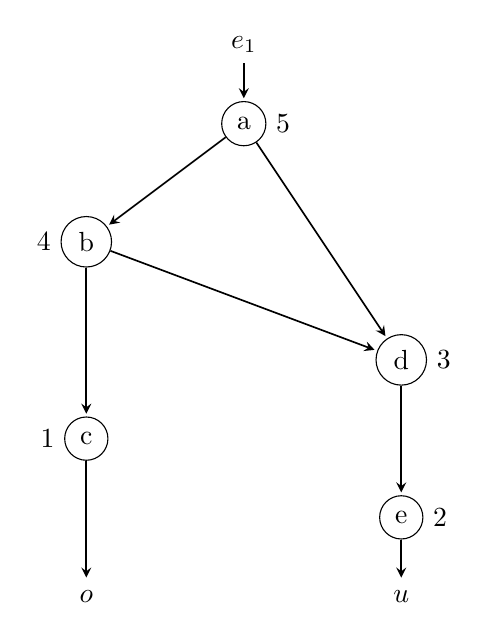
\begin{tikzpicture}
    [pre/.style={<-,shorten <=1pt,>=stealth,semithick}]
    \node (s) at (2,5) {\(e_1\)};
    \node [shape=circle,draw=black] (a) [label=right:5] at (2, 4) {a}
      edge [pre] (s);
    \node [shape=circle,draw=black] (b) [label=left:4] at (0,2.5) {b}
      edge [pre] (a);
    \node [shape=circle,draw=black] (c) [label=left:1] at (0,0) {c}
      edge [pre] (b);
    \node [shape=circle,draw=black] (d) [label=right:3] at (4,1) {d}
      edge [pre] (a)
      edge [pre] (b);
    \node [shape=circle,draw=black] (e) [label=right:2] at (4,-1) {e}
      edge [pre] (d);
    \node (o1) at (0,-2) {\(o\)} edge [pre] (c);
    \node (o2) at (4,-2) {\(u\)} edge [pre] (e);
  \end{tikzpicture}
  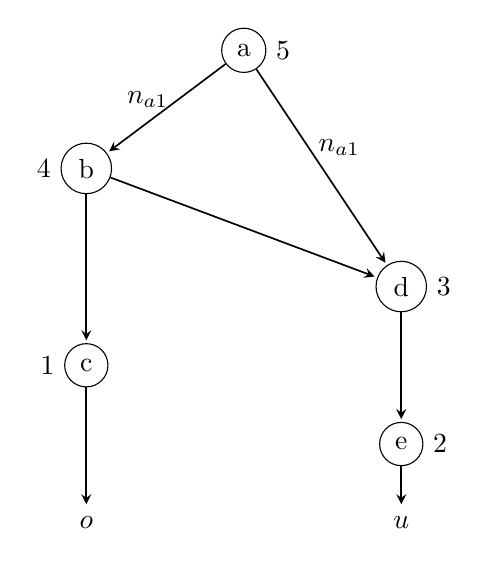
\begin{tikzpicture}
    [pre/.style={<-,shorten <=1pt,>=stealth,semithick}]
    \node [shape=circle,draw=black] (a) [label=right:5] at (2, 4) {a};
    \node [shape=circle,draw=black] (b) [label=left:4] at (0,2.5) {b}
      edge [pre] node[align=left,left,pos=0.6] {\(n_{a1}\)} (a);
    \node [shape=circle,draw=black] (c) [label=left:1] at (0,0) {c}
      edge [pre] (b);
    \node [shape=circle,draw=black] (d) [label=right:3] at (4,1) {d}
      edge [pre] node[align=right,right,pos=0.6] {\(n_{a1}\)} (a)
      edge [pre] (b);
    \node [shape=circle,draw=black] (e) [label=right:2] at (4,-1) {e}
      edge [pre] (d);
    \node (o1) at (0,-2) {\(o\)} edge [pre] (c);
    \node (o2) at (4,-2) {\(u\)} edge [pre] (e);
  \end{tikzpicture}
  \caption{Visualization of a simple asynchronous system with a reversed topological order.}
\label{fig:chap3:sec_sync:visual_dag}
\end{figure}

Figure~\ref{fig:chap3:sec_sync:visual_dag} visualizes a synchronous evaluation engine.
It shows two \glspl{dag} representations of an evaluation engine  where the nodes a to e are labeled in a reversed topological order and \(o\) and \(u\) represents the output streams with that name.
The left system is in its initial state and an input event \(e_1\) is present and can be consumed by the input node a.
When a node is chosen to compute by the scheduler, only node a is enabled, therefore it is scheduled.
The right system is the representation of the next step: node a has consumed the external event and produced an internal event \(n_{a1}\), which is propagated to all it's children: node b and d.
In the next step node b would be scheduled, because it has the lowest number of any node that can compute (actually it's the only node that can compute at all, because d has to wait for the event from b).
After b was scheduled, it would have produced the internal event \(n_{b1}\) which would then be distributed to nodes c and d.

The complete run of the synchronous engine for one input is the following, where the states are not further defined:

\begin{align*}
  \langle
    (\lambda,                             s_0),
    ((\{ n_{a1}         \}, \{n_{b1}\}),  s_1),
    ((\{ n_{b1}         \}, \{o_1\}),     s_2),\\
    ((\{ n_{a1}, n_{b1} \}, \{n_{d1}\}),  s_3),
    ((\{ n_{d1}         \}, \{u_1\}),     s_4)
  \rangle
\end{align*}

If there were more then one input event, at this point node a would be scheduled again.
It would consume the next external event and the following nodes would be scheduled in the same order as before, extending the run in an obvious way.

\subsection{Asynchronous Evaluation}
\label{sec:concepts:behaviour_without_timing:async}

An asynchronous evaluation engine is one with a fair, but not fixed schedule.

In contrast to the synchronous evaluation engine it has no fixed schedule, the only requirement is that the schedule is fair.
Therefore predecessors of enabled nodes can perform multiple computations before their children are scheduled and events are not \emph{pushed} through the \gls{dag} as fast as possible.
\todo{more later}

\section{Equivalence of Different Schedules Without Timing Functions}
\label{sec:concepts:equivalence_without_timing}

Based on the described behaviours of the approaches we now can proof the equivalence of different schedules for the same evaluation engine for a \gls{tessla} specification.

\begin{lemma}[name = Equivalence of Engines for one Input]\label{lemma:eval_equivalent_if_runs_equal}
  Two evaluation engines are equivalent for an input, if their runs are equivalent for that input.
\end{lemma}

\begin{proof}
  Since two runs are equal if they have the same last state, and all events which were produced are stored in the state, during both runs the same output events had to be generated or else their state would differ.
\end{proof}

As defined by definition~\ref{def:valid_eval_engine} any evaluation engine has to be equivalent to a synchronous one to be valid.

The equivalence is shown in two steps: first in Section~\ref{sec:concepts:equivalence_without_timing:synchronous} it is shown, that all possible synchronous engines for a specification are equivalent, so there is only one valid evaluation for a specification over a fixed input.
Afterwards in Section~\ref{sec:concepts:equivalence_without_timing:sync_async} it is shown that any asynchronous evaluation engine is equivalent to a synchronous one.


\subsection{Equivalence of Synchronous Systems}
\label{sec:concepts:equivalence_without_timing:synchronous}

When given a series of input events, two synchronous evaluation engines for a specification with different schedules will have different runs.
But both will produce all outputs that can be produced after consuming one specific input before the next input is consumed as reasoned in Section~\ref{sec:concepts:behaviour_without_timing:synchronous}.
Also both runs will obviously have the same length (both engines are the same \gls{dag}, so they have the same number of nodes), let that length be \(l\).

To proof the equivalence of both engines we can prove the equivalence of their runs.
To show the equivalence we will show that there is always another run, which is equivalent to the second one, that is closer to the first one.
If such a closer run always exist, we will show that the run with closeness \(l, 0\) to the first run, which has to be the first run itself, is also an equivalent run to the second run.

\begin{theorem}[name = Equivalence of Different Synchronous Evaluation Engines]\label{theorem:equivalence_sync_eval_engines}
  Two synchronous evaluation engines for a specification with different schedules are equivalent.
\end{theorem}
\begin{proof}

  Let \(r_1, r_2\) be the runs of the two engines for a given \gls{tessla} specification.
  Because each \gls{tessla} specification contains only a finite amount of functions and works on finite traces, the runs also have to be finite.

If the two runs aren't equal, they must have a closeness which is smaller than \((l, 0)\).
Let \([r_2]\) be the set of all runs that are equivalent to \(r_2\).
All of those runs will also have a closeness from \(r_1\) which is smaller than \((l, 0)\).
Select one run \(r_2' \in [r_2]\) which has a minimal closeness from \(r_1\).
Let \((d,k) = \delta(r_1, r_2')\).

This means that at step \(d\) the run \(r_2'\) has taken a different transition than run \(r_1\).
Let the transitions the runs have taken be \(\tau_1\) for \(r_1\) and \(\tau_2\) for \(r_2'\).
Run \(R_2'\) will take transition \(\tau_1\) at step \(d+k\) (as per the definition of the closeness).
Obviously the two transitions have to be independent of each other, else they couldn't have been taken in different order by the two runs.

If \(k > 1\) there will be a transition \(\tau_2' \neq \tau_1\) which is taken by the run \(r_2'\) at step \(d+(k-1)\).
While this transition \(\tau_2'\) must also be taken in the first run as per Lemma~\ref{lemma:enabled_till_scheduled}, it's not possible, that it was taken before \(\tau_1\), beause then the two runs wouldn't have been the same upto the point where \(\tau_1\) was taken.
Therefore \(\tau_1\) has to be independent of \(\tau_2'\), and because \(\tau_2'\) was scheduled by the second run before \(\tau_1\) both transitions are independent of each other.

As of Lemma~\ref{lemma:independent_nodes} which one of them is taken first can't change the enabledness of the node of the second transition.
Therefore there is a run \(r_2''\), which is equal to \(r_2'\), except that the transitions \(\tau_1, \tau_2'\) are scheduled the other way around.
Figure~\ref{fig:chap3:sec_sync:commutativity_scheduling} visualizes how changing the order of the two transitions can't change the global state of the engine after both were taken.
Therefore the runs \(r_2'\) and \(r_2''\) are equivalent and their closeness to \(r_1\) is \(d, k-1\), which contradicts the initial statement that \(r_1'\) was a run with a maximal closeness.
This means that there is an equivalent run to \(r_2\) which has at least the closeness \((d, 1)\).

If \(k = 1\) the transition \(\tau_2'\) from the previous case is equal to \(\tau_2\).
Based on the same reasoning there also exist a run \(r_2''\) which is equal to \(r_2'\), except that the order of \(\tau_2\) and \(\tau_1\) is changed, and which is also equivalent to \(r_2'\) and to \(r_2\).
This run has the closeness \((d, 0)\) to \(r_1\).
This obviously doesn't make sense: The first element of the closeness is the last step where both runs are equal, the second element describes how many steps afterwards the differing transition was taken.
But if it was taken right in the step after the last equal step, there is no difference at that position, so the closeness of \(r_1\) and \(r_2''\) can be at least \((d+1, x), x \in \mathbb{N}_{>0}\).
This also contradicts our initial statement that \(r_2'\) was the run with the biggest closeness to \(r_1\) which is equivalent to \(r_2\).

Combined we can now say, that there is no upper bound on the closeness of equivalent runs of \(r_2\) to \(r_1\), therefore the run with the closeness \((l, 0)\) also has to be equivalent to \(r_2\).

\end{proof}


\begin{figure}
  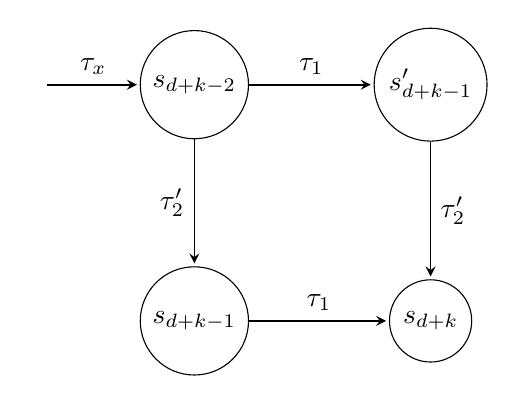
\begin{tikzpicture}
    [pre/.style={<-,shorten <=1pt,>=stealth,semithick}]
    \node (A) at (0,0) {};
    \node [shape=circle,draw=black] (B) at (2, 0) {\(s_{d+k-2}\)}
      edge [pre] node[above] {\(\tau_{x}\)} (A);
    \node [shape=circle,draw=black] (C) at (2, -3) {\(s_{d+k-1}\)}
      edge [pre] node[left] {\(\tau_{2}'\)} (B);
    \node [shape=circle,draw=black] (D) at (5, 0) {\(s_{d+k-1}'\)}
      edge [pre] node[above] {\(\tau_{1}\)} (B);
    \node [shape=circle,draw=black] (E) at (5, -3) {\(s_{d+k}\)}
      edge [pre] node[right] {\(\tau_{2}'\)} (D)
      edge [pre] node[above] {\(\tau_{1}\)} (C);
  \end{tikzpicture}
  \caption{Commutativity Diagramm of Node scheduling}
\label{fig:chap3:sec_sync:commutativity_scheduling}
\end{figure}



\subsection{Equivalence of Synchronous and Asynchronous Schedules}
\label{sec:concepts:equivalence_without_timing:sync_async}

When the nodes of \(a\) aren't scheduled in reversed topological order, the system can consume inputs before producing all outputs based on the last consumed input.
Therefore the reordering of runs has to be performed over wider parts of the run.
% Idea: each step is a commutation of two internal events in regard to the rev top order.
% => show commutativity of traces (note: only valid commutations, no two events, where one depends one the other, can be commuted, this is ensured by the scheduling of nodes that have input buffered)

\section{Behaviour with Timing functions}
\section{Equalitys with Timing functions}
\section{Parallel computation}
 % INCLUDE: concepts
% % !TEX root = ../thesis-example.tex
%
\chapter{Conclusion}
\label{sec:conclusion}

Citation test~\cite{Pike2010}
 % INCLUDE: conclusion
\cleardoublepage

% --------------------------
% Back matter
% --------------------------
{%
    \setstretch{1.1}
    \renewcommand{\bibfont}{\normalfont\small}
    \setlength{\biblabelsep}{0pt}
    \setlength{\bibitemsep}{0.5\baselineskip plus 0.5\baselineskip}
    \printbibliography[nottype=online]
    \printbibliography[heading=subbibliography,title={Webseiten},type=online,prefixnumbers={@}]
}
\cleardoublepage

\listoffigures
\cleardoublepage

\listoftables
\cleardoublepage

% !TEX root = ../thesis.tex
%
\pagestyle{empty}
\hfill
\vfill
\pdfbookmark[0]{Colophon}{Colophon}
\section*{Colophon}

This thesis was typeset with \LaTeXe.
It uses the \textit{Clean Thesis} style developed by Ricardo Langner.
The design of the \textit{Clean Thesis} style is inspired by user guide documents from Apple Inc.

Download the \textit{Clean Thesis} style at \url{http://cleanthesis.der-ric.de/}.

\cleardoublepage

% !TEX root = ../thesis-example.tex
%
%************************************************
% Declaration
%************************************************
\pdfbookmark[0]{Declaration}{Declaration}
\chapter*{Declaration}
\label{sec:declaration}
\thispagestyle{empty}
\vfill

Ich versichere an Eides statt, die vorliegende Arbeit selbstständig und nur unter Benutzung der angegebenen Quellen und Hilfsmittel angefertigt zu haben.
\bigskip

\noindent\textit{\thesisUniversityCity, \thesisDate}

\smallskip

\begin{flushright}
    \begin{minipage}{5cm}
        \rule{\textwidth}{1pt}
        \centering{\thesisName}
    \end{minipage}
\end{flushright}

%*****************************************
%*****************************************

\clearpage
\newpage
\mbox{}

% **************************************************
% End of Document CONTENT
% **************************************************
\end{document}
